\chapter{Results \& Discussion}
This chapter presents the evaluation of the developed end-to-end autonomous navigation system. The results are presented chronologically, tracing the system's iterative development. All physical deployment and inference runs reported in this chapter were executed on the real robot, with the trained model running onboard a Raspberry Pi embedded on the platform.

To validate the necessity of the final image preprocessing architecture, the chapter first details the offline training and real-world physical testing of two early experimental baselines. By analyzing the specific failure modes of these early iterations, the empirical justification for the proposed Egocentric Dynamic Crop Model is established.


\section{Chronological Development and Experimental Baselines}
During the development of the navigation framework, the state representation of the track underwent three major iterations. All models were trained using a modified NVIDIA DAVE-2 Convolutional Neural Network (CNN) architecture with 2,211,175 parameters, processing $200 \times 200$ pixel images, and minimizing Mean Squared Error (MSE) using the Adam optimizer.

\subsection{Iteration 1: Baseline A (Allocentric Full AOI Model)}
The initial approach utilized the raw, top-down Bird's-Eye View (BEV) image, retaining the room's floor textures and permanent background elements.

During offline training, Baseline A converged rapidly. As shown in Figure~\ref{fig:4.1}, both MSE and MAE decreased exponentially, with validation loss plateauing near 0.05 and 0.13, and reaching a low validation MSE of 0.0489 by Epoch 30.

% [Insert Figure 4.1: Baseline A (Allocentric Full AOI) Offline Training and Validation Loss Curves]
\begin{figure}[htbp]
	\centering
	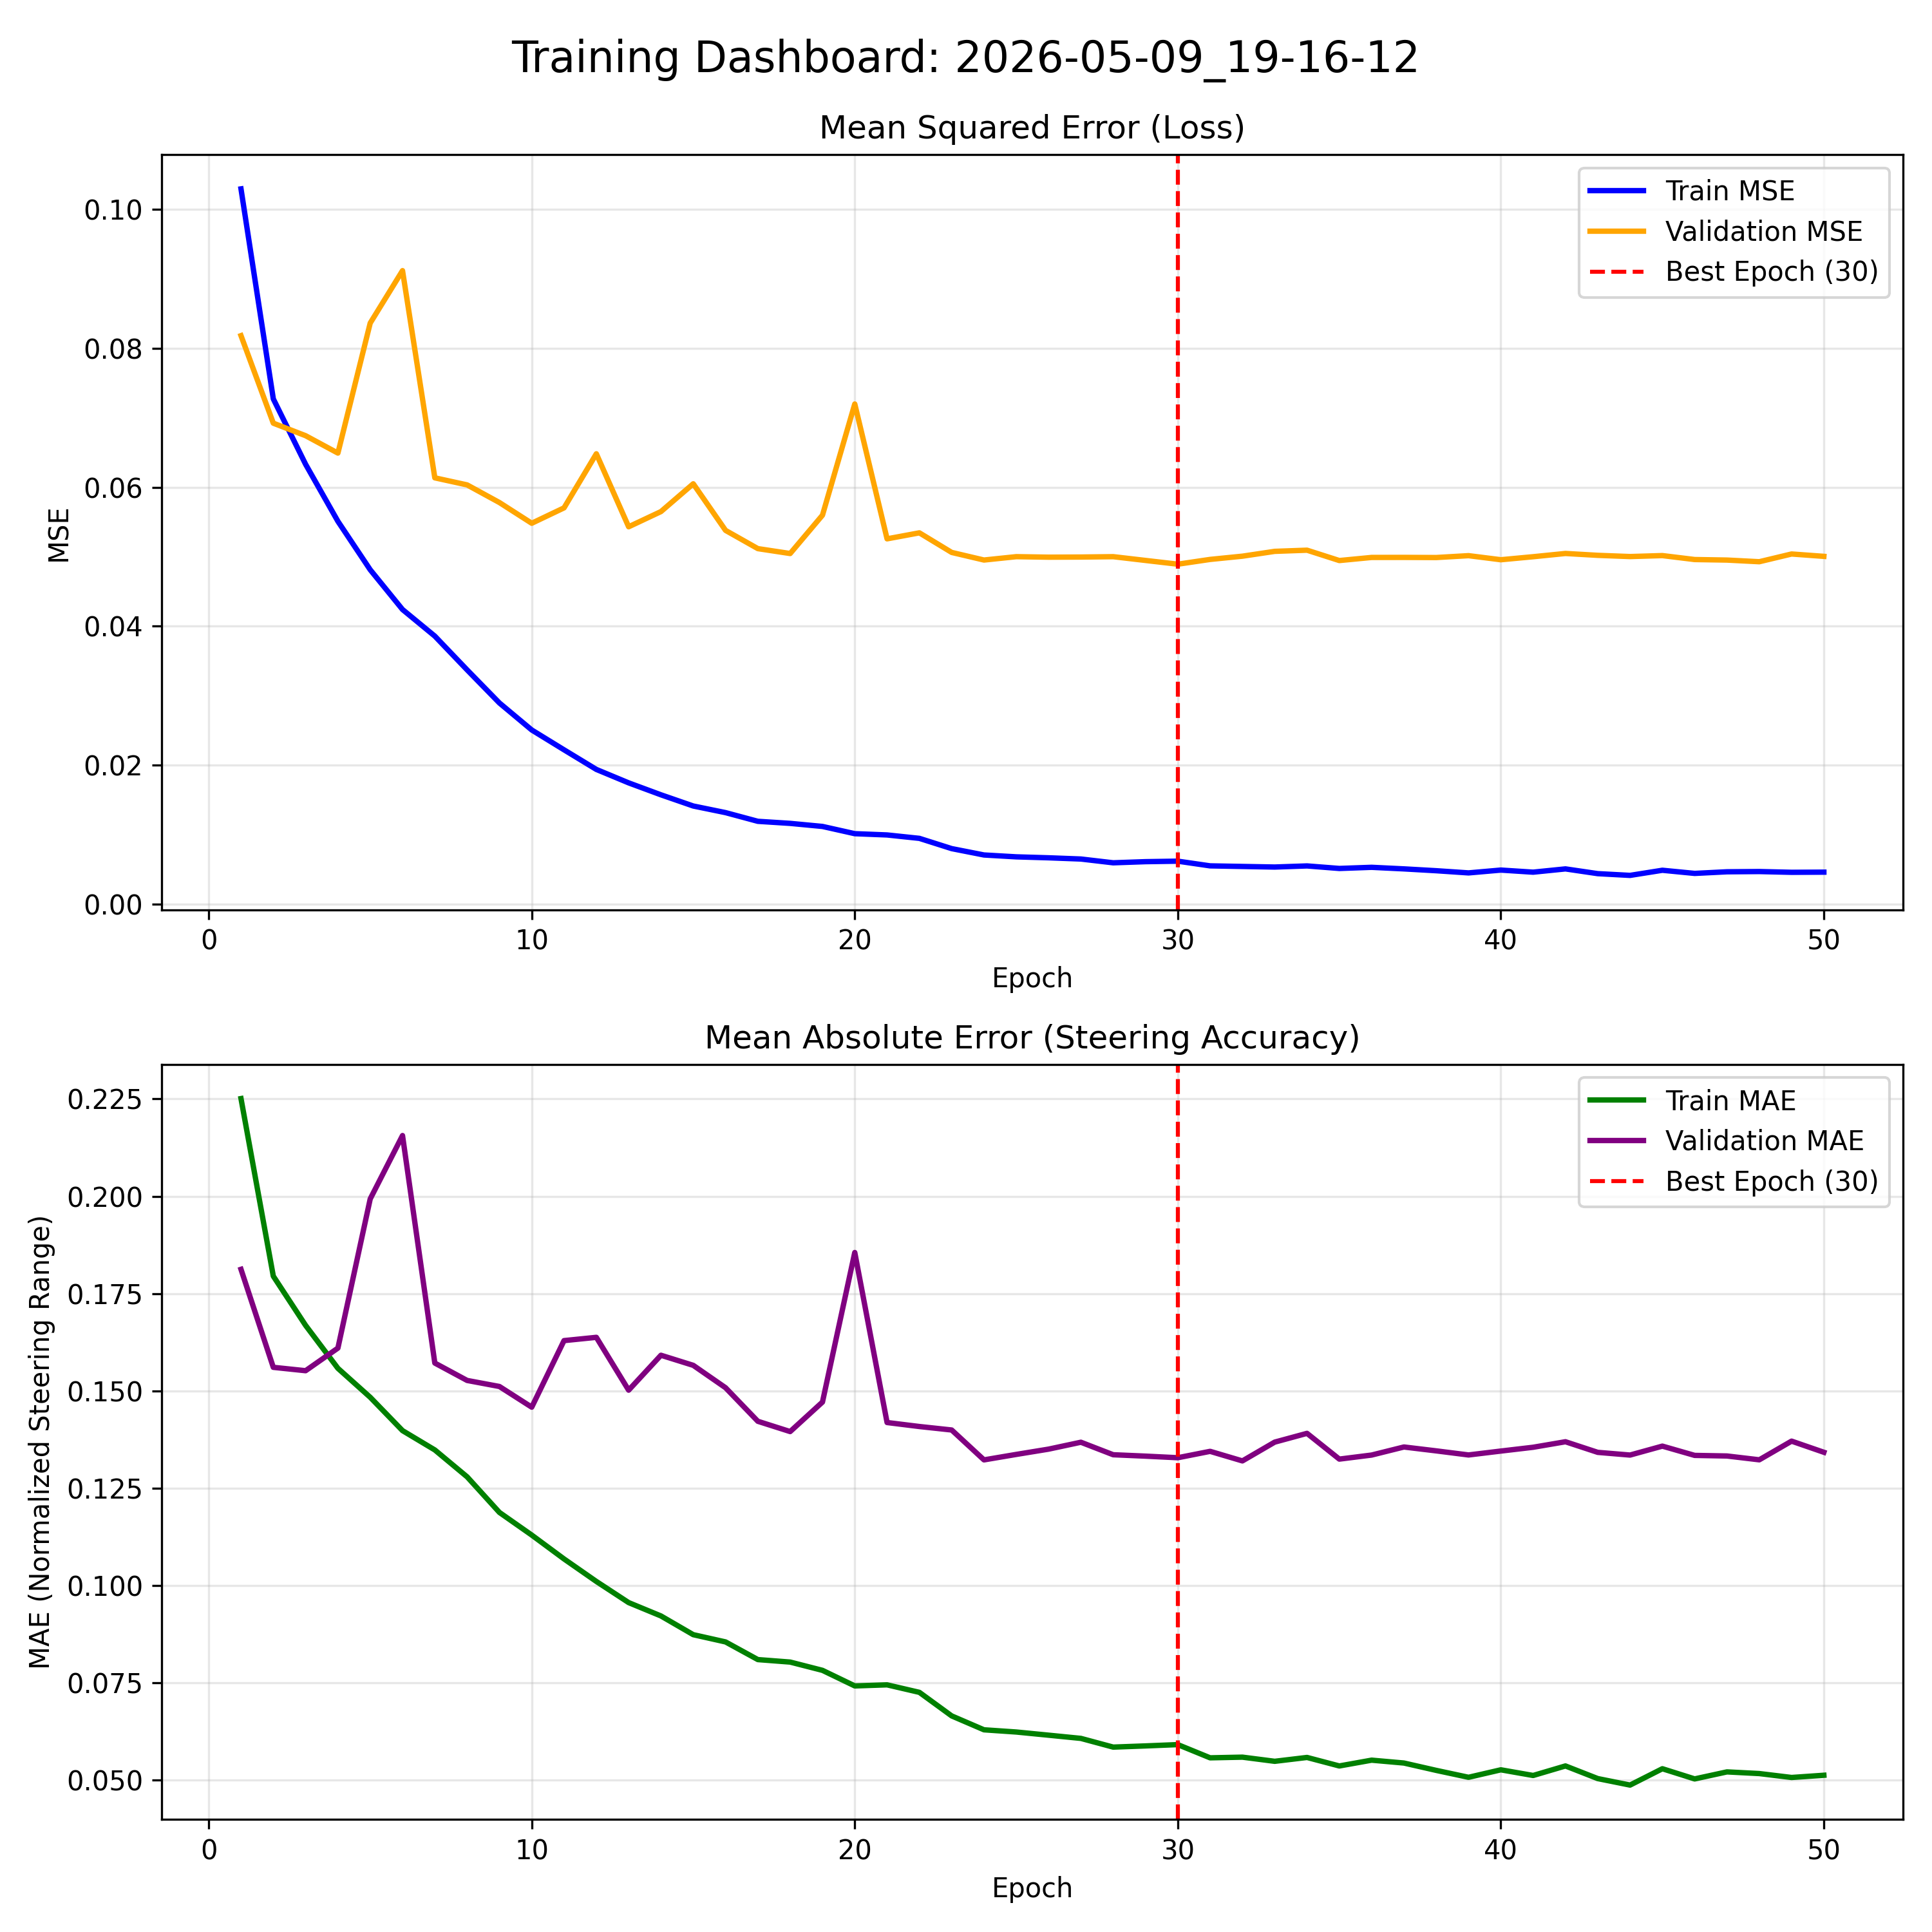
\includegraphics[width=1\linewidth]{chap4/images/2nd_session.png}
	\caption{The near-perfect convergence of MSE and MAE suggested successful learning, though this was later identified as spatial memorization.}\label{fig:4.1}
\end{figure}

However, physical deployment resulted in immediate, catastrophic navigation failure. On the physical track, the robot exhibited erratic motor control, immediately veering off-path and breaching the arena boundaries.

\begin{figure}[htbp]
	\centering
	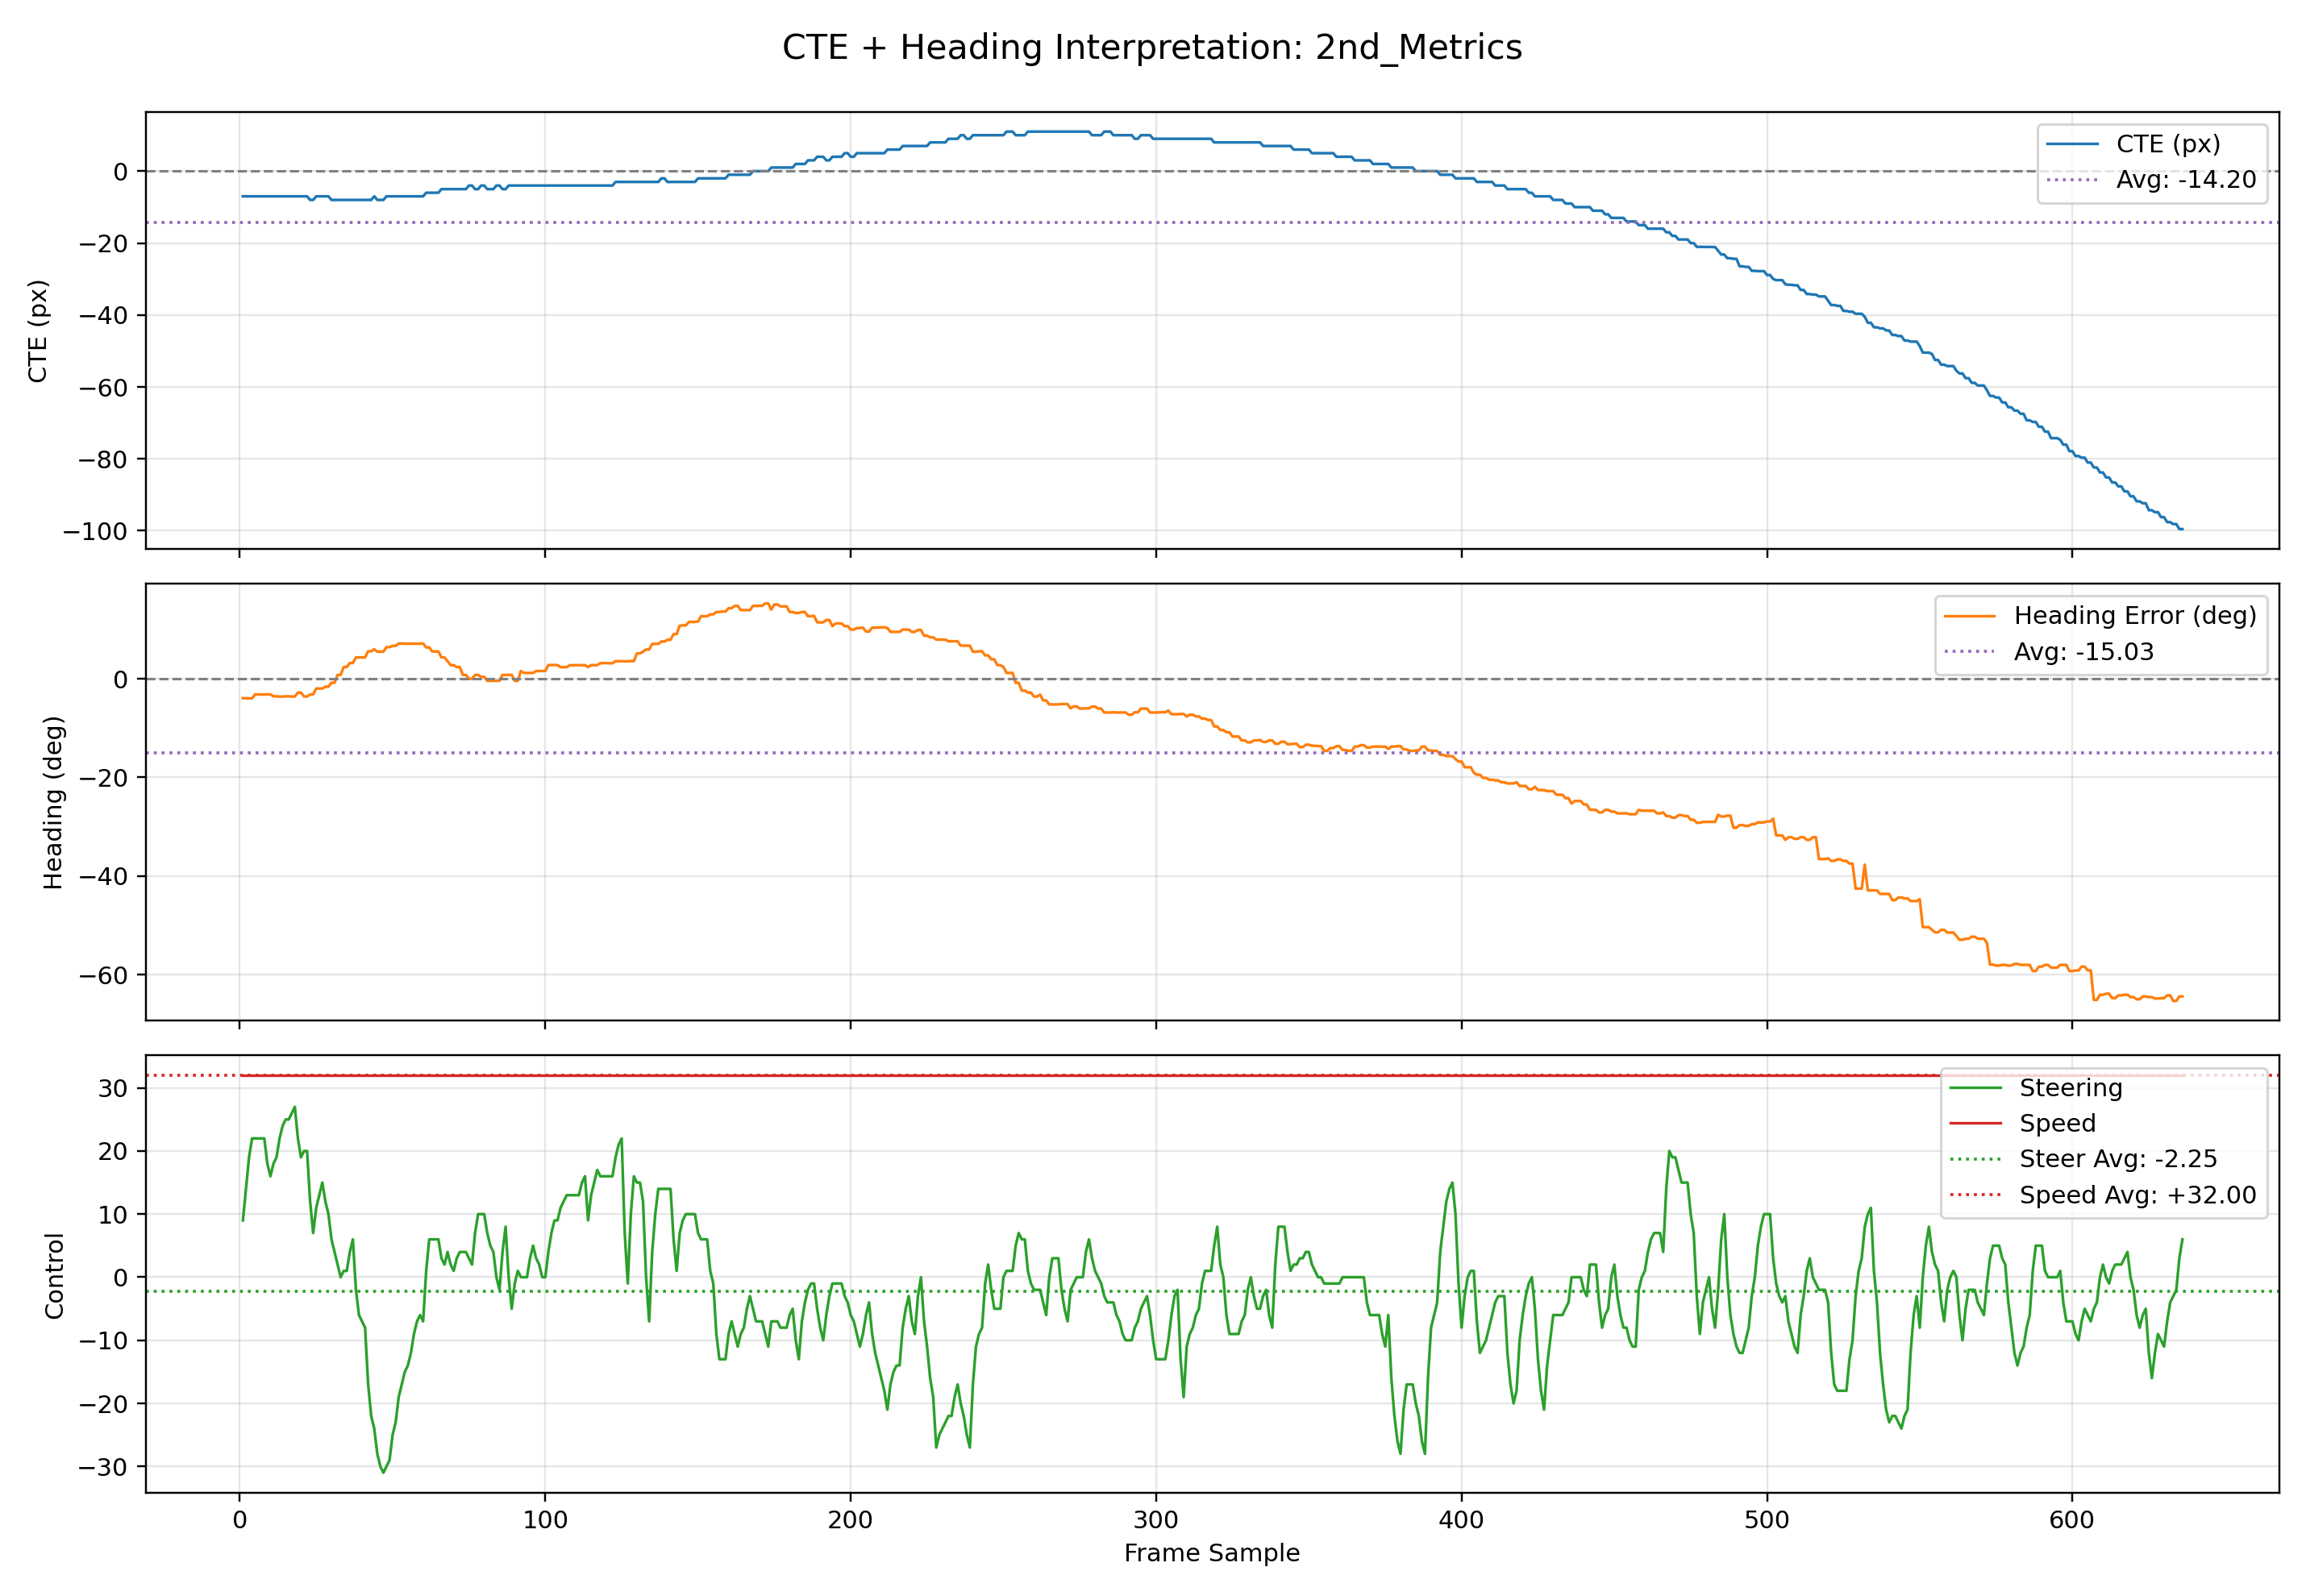
\includegraphics[width=1.0\linewidth]{chap4/images/2nd_Metrics_interpretation.png}
	\caption{Physical deployment of the Allocentric Full AOI Model resulted in immediate navigation failure.}\label{fig:4.2}
\end{figure}

As shown in Figure~\ref{fig:4.2}, both the Cross-Track Error (CTE) and the Heading Error ($\theta_{err}$) diverged immediately on deployment (CTE quickly exceeding $-100$ pixels and Heading Error dropping past $-60^\circ$). Baseline A maintained the path for only 636 frames with an RMSE of 30.9992 pixels. When analyzing the Error Compounding Rate over the first 500 frames, Baseline A showed rapid, exponential error growth. Minor starting position changes on the real track confused the network, causing it to immediately steer off course.

Post-deployment analysis revealed the model suffered from \textbf{shortcut learning}. Because the room environment and global track remained static in the camera's view, the CNN bypassed learning the path geometry entirely. Instead, it overfit directly to the robot's absolute pixel coordinates within the room frame. The validation error remained low during training because validation images came from that same static frame. During inference, any minor starting deviation created an out-of-distribution pixel state that the model could not interpret.

\subsection{Iteration 2: Baseline B (Feature-Extracted Allocentric Model)}
To eliminate background shortcuts like floor reflections, shadows, and pixel discrepancies, the pipeline was updated to add a semantic polygon extraction step. This process isolated the AOI as flat white shapes with a red polygon on a pure black canvas, removing all environmental noise and forcing the network to learn the path geometry itself.

While this removed environmental noise, offline training metrics immediately destabilized. As shown in Figure~\ref{fig:4.3}, the training profile exhibited severe validation noise and a massive loss spike near epoch 13, indicating the network struggled to map steering angles without its familiar background shortcuts. The resulting controller was not stable enough to justify full physical deployment, and the model was therefore not advanced beyond limited sanity checks.


\begin{figure}[H]
	\centering
	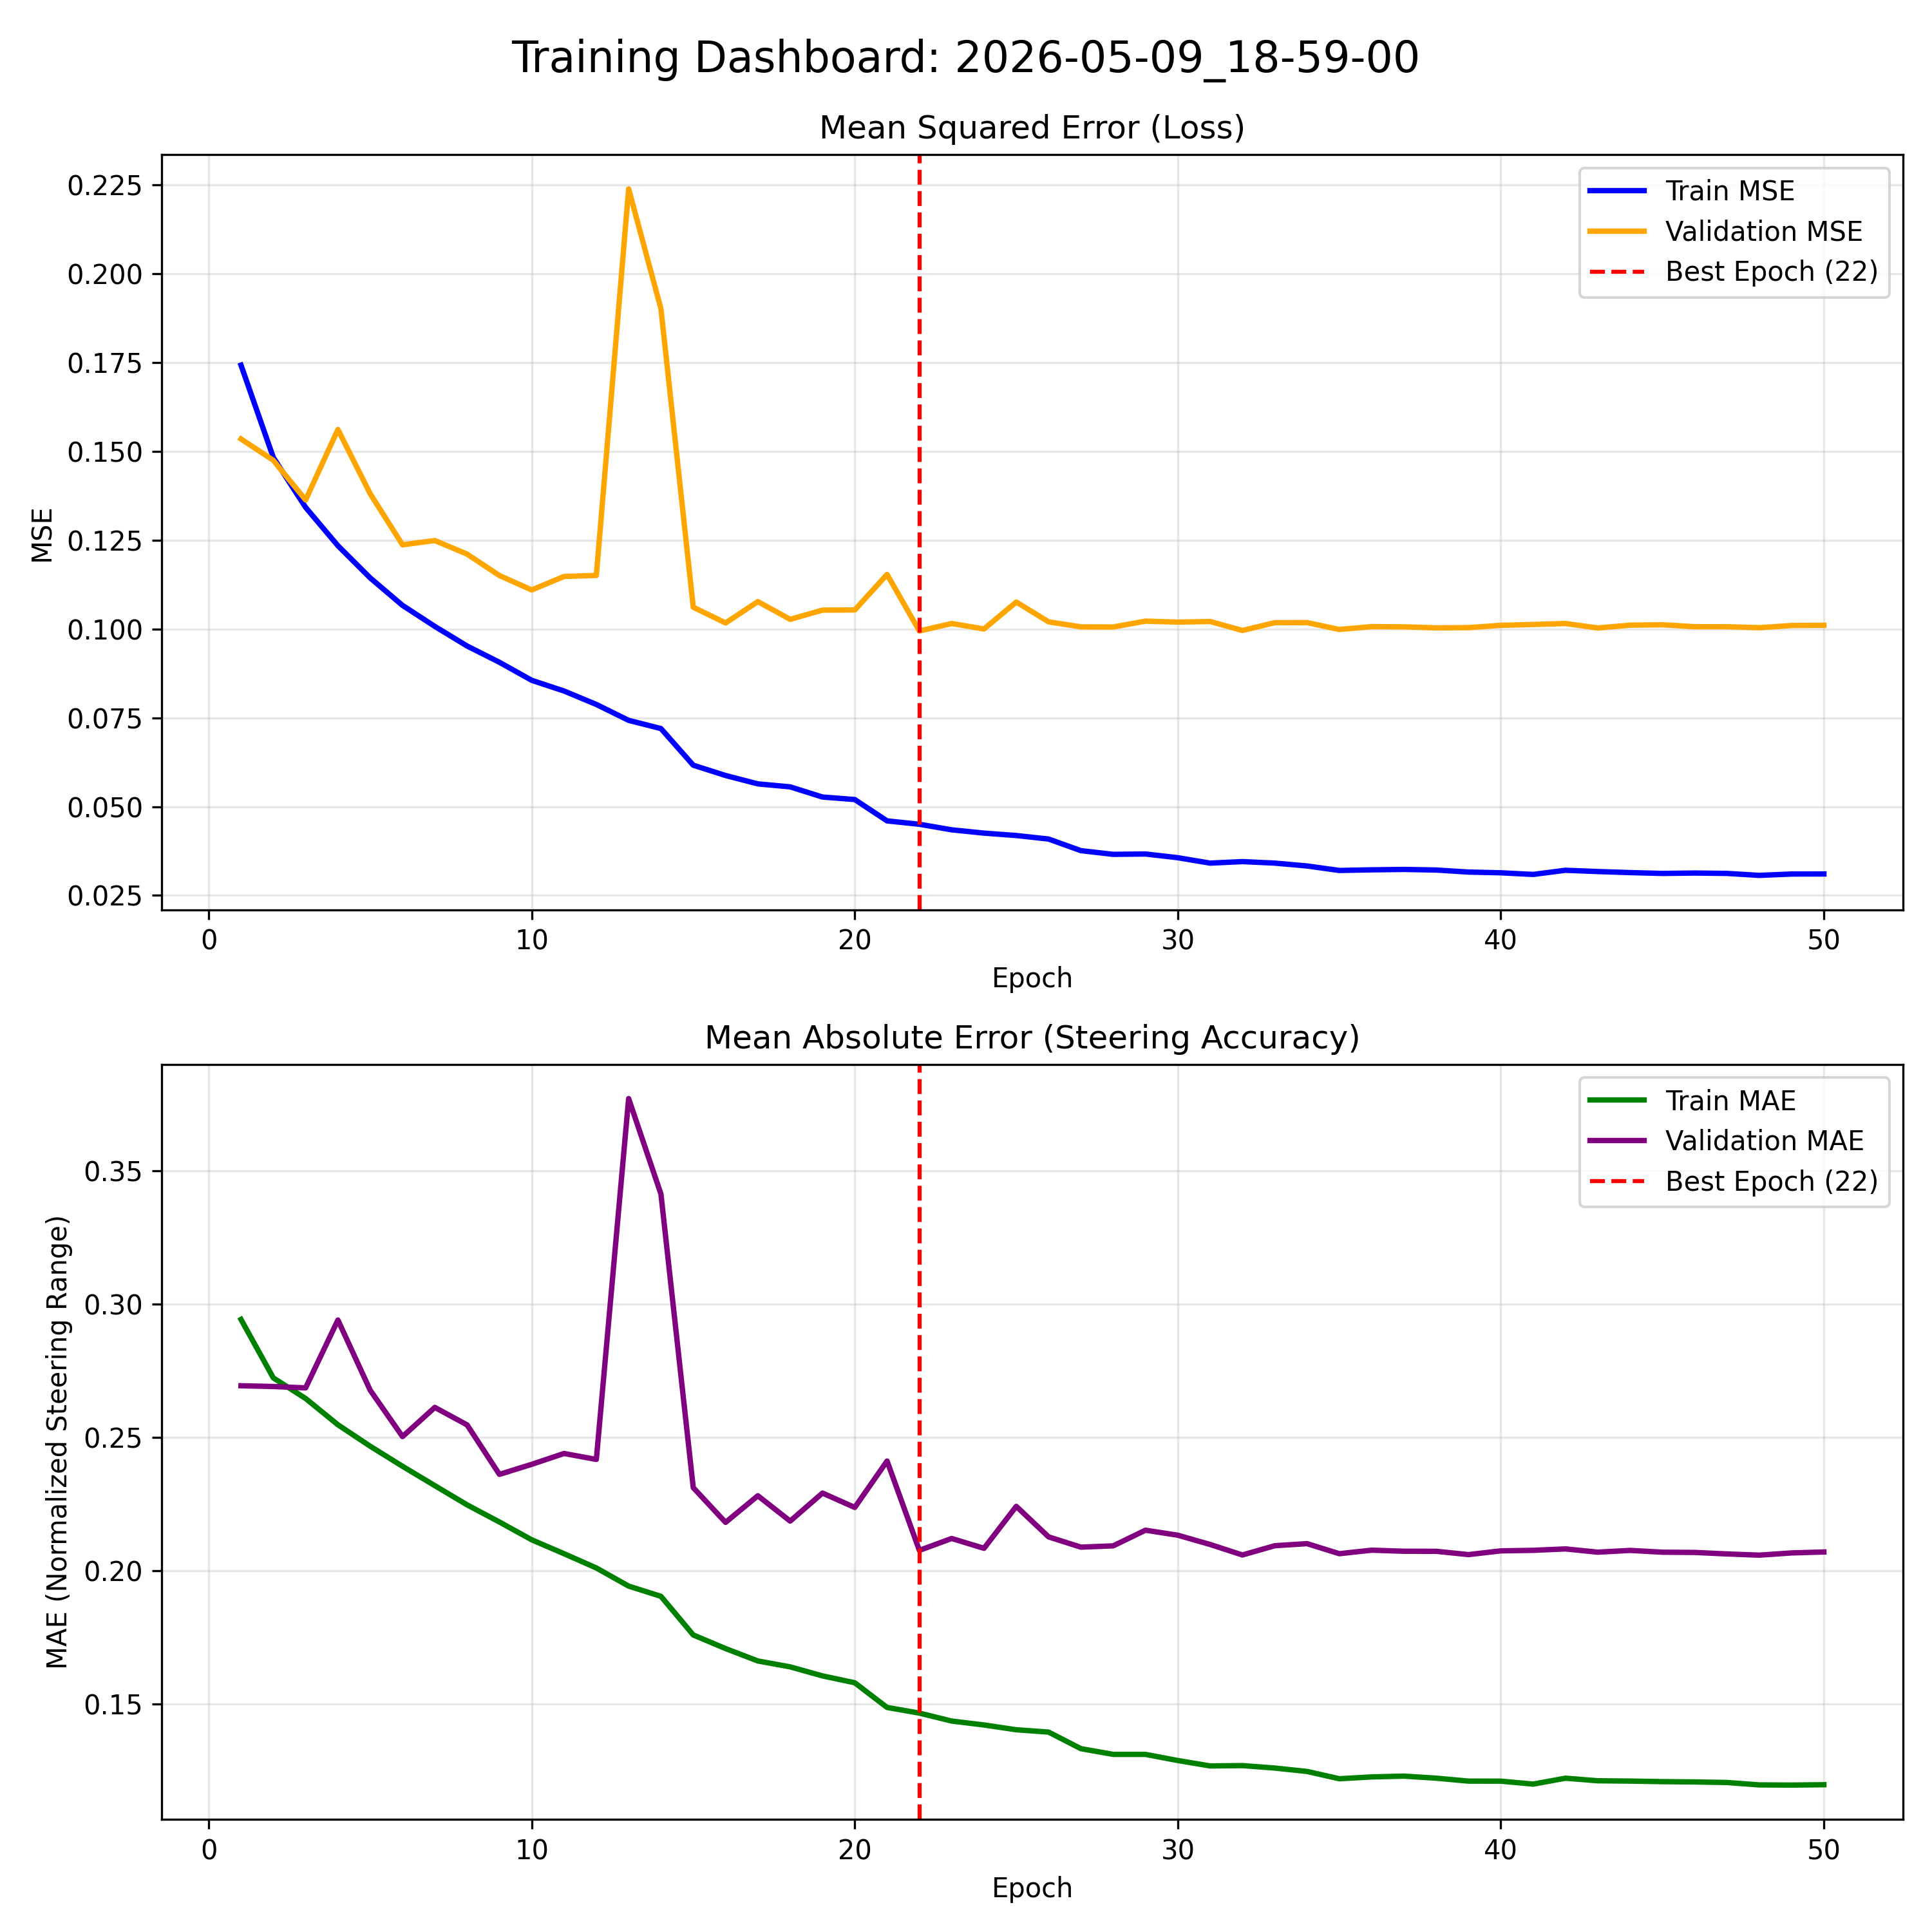
\includegraphics[width=1.0\linewidth]{chap4/images/4th-session.png}
	\caption{The Feature-Extracted Allocentric Model's training profile was unstable, with severe validation noise and a massive loss spike, indicating the network struggled without background shortcuts.}\label{fig:4.3}
\end{figure}

Limited real-world trials at reduced speed still exposed the same instability. The failure was reproduced across two separate deployment sessions, in which the controller survived only 772 and 1{,}122 frames with CTE RMSE values of 35.72~px and 84.38~px respectively (Table~\ref{tab:4.1}), confirming that the instability was systematic rather than an isolated event. As shown in Figure~\ref{fig:4.4} for the longer session, the Cross-Track Error (CTE) drifted steadily upward to roughly 80 pixels before collapsing, while the Heading Error hovered around $-20^\circ$ and then jumped abruptly to approximately $+60^\circ$ near the failure point. The steering signal oscillated with a near-zero mean while speed was increased, indicating the controller was reacting to noise rather than tracking a stable path.

\begin{figure}[H]
	\centering
	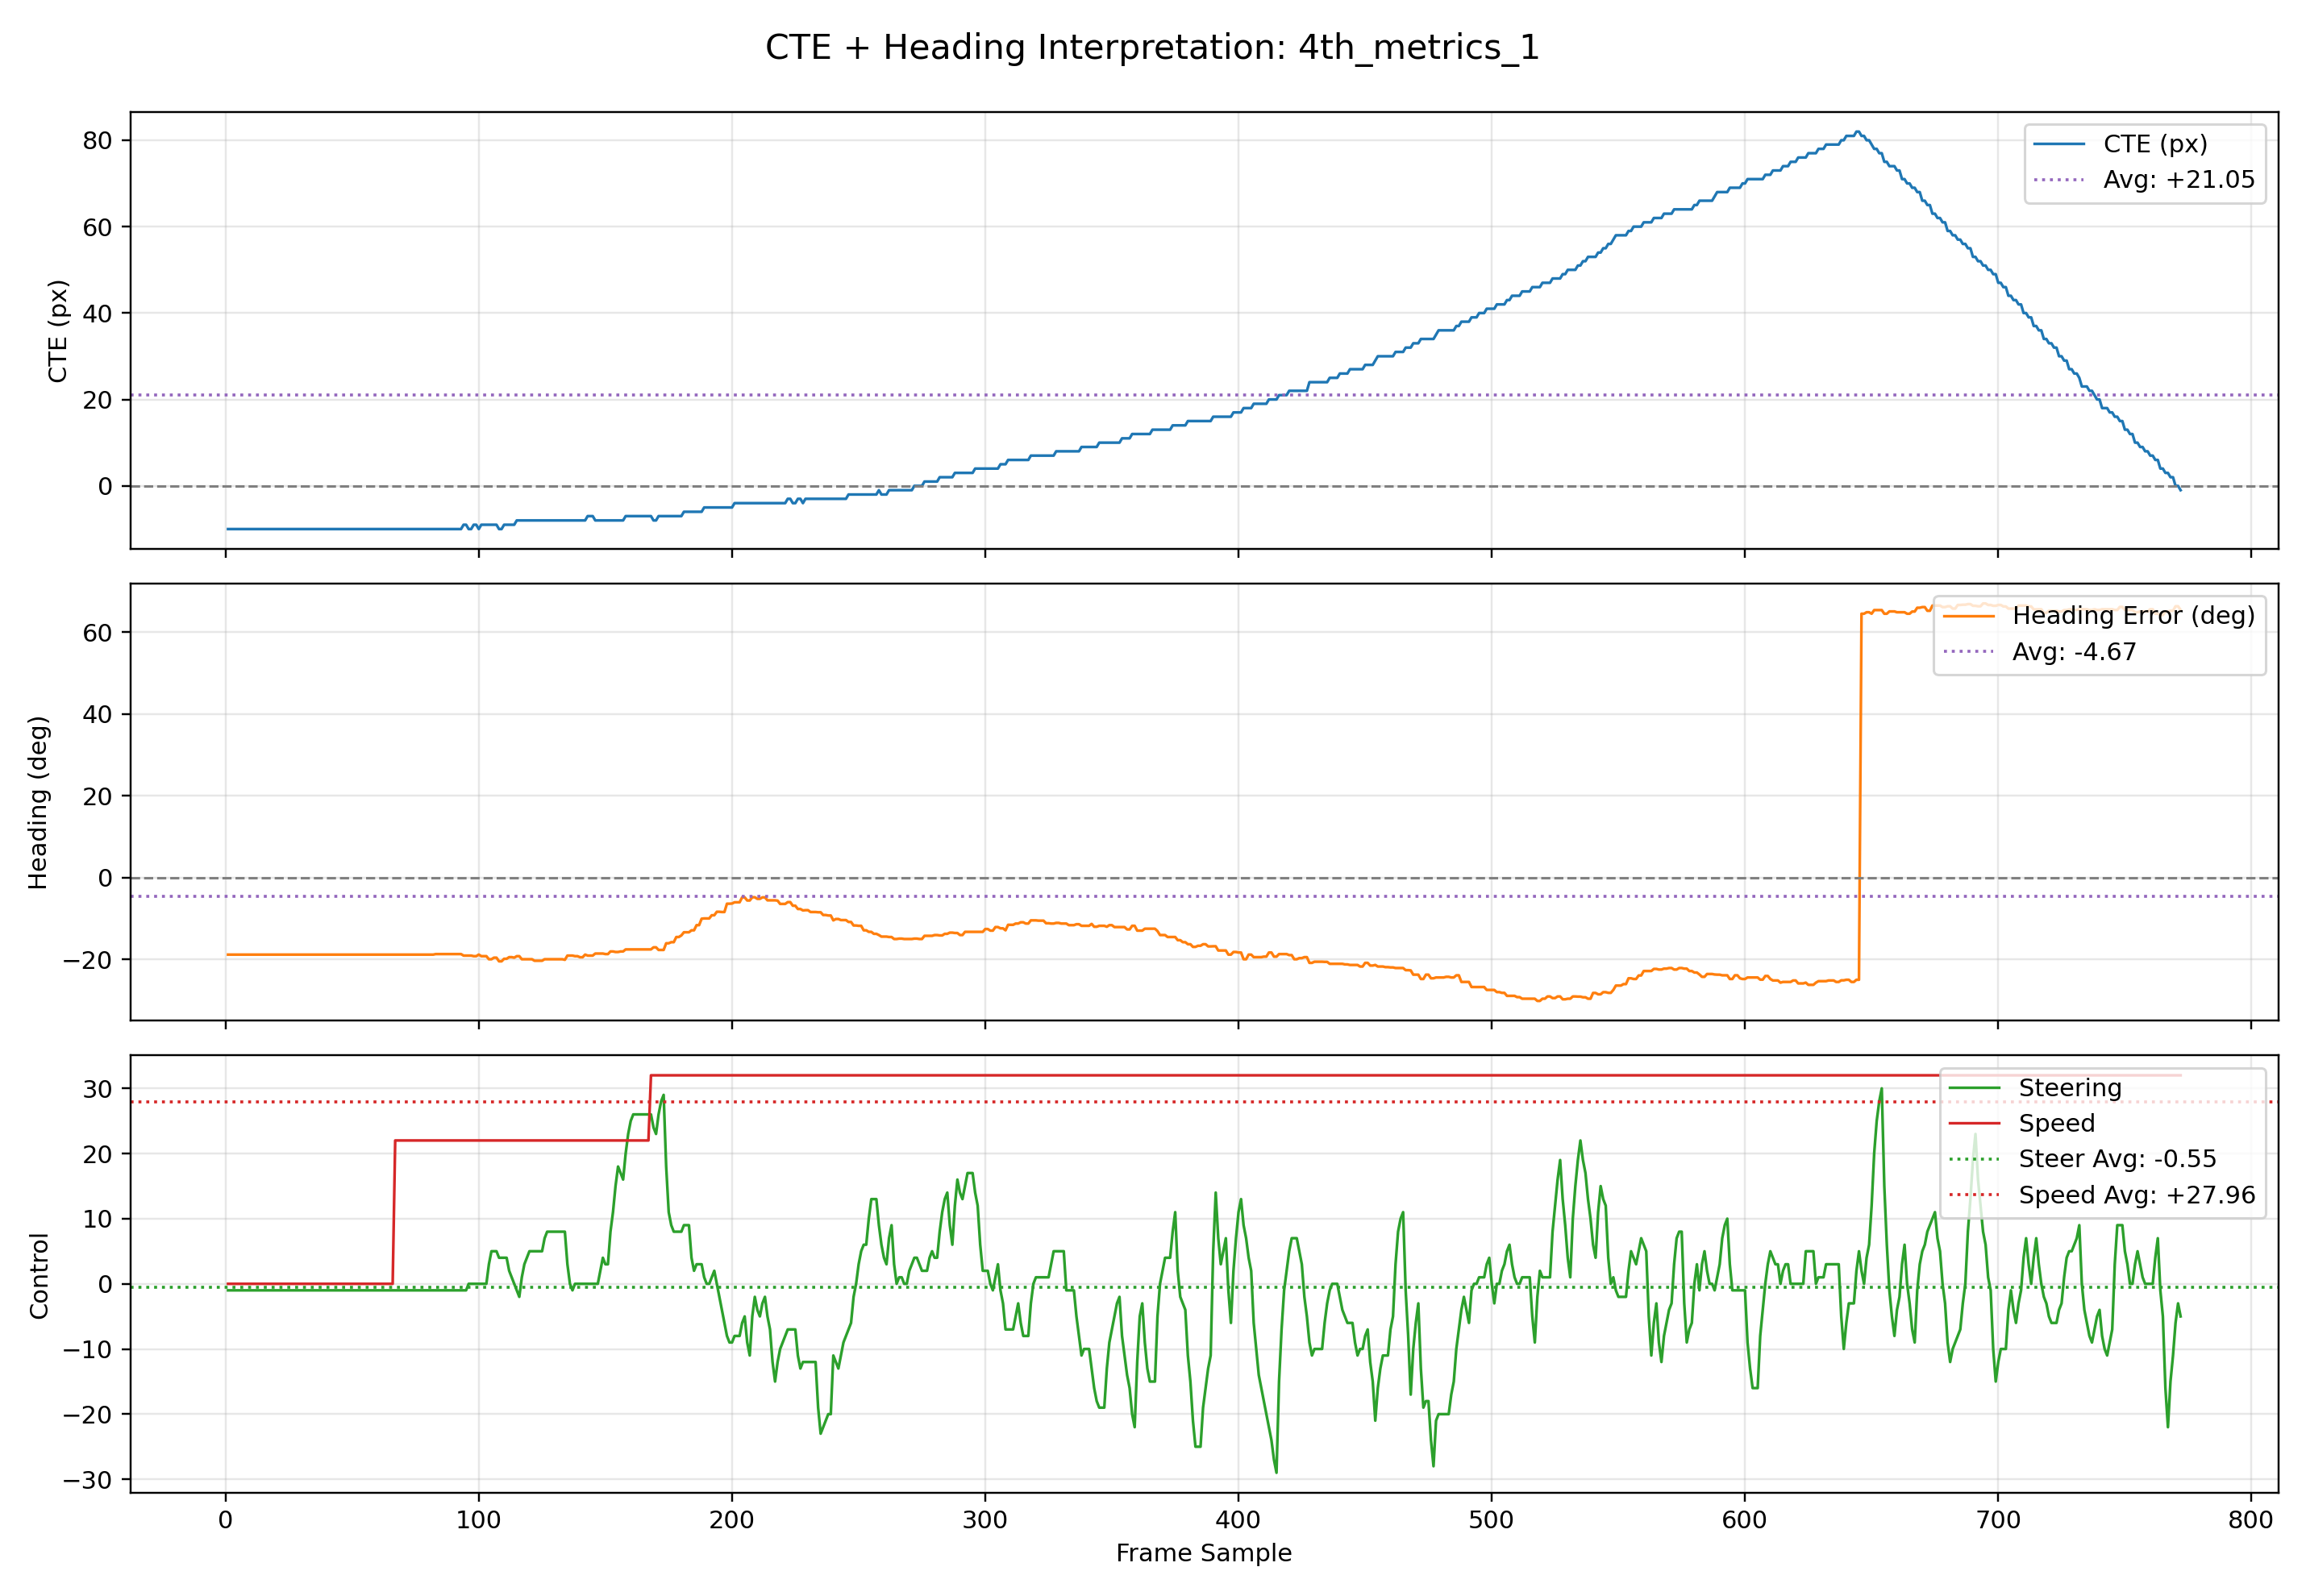
\includegraphics[width=1.0\linewidth]{chap4/images/4th_metrics_1_interpretation.png}
	\caption{Limited real-world trial for Baseline B. CTE drifted upward with a late-stage heading discontinuity, while steering oscillations persisted under increasing speed.}\label{fig:4.4}
\end{figure}

\subsection*{Failure Analysis of Baselines A and B}
The two allocentric baselines failed for complementary reasons that both trace back to the state representation. Baseline A preserved the full room context, which enabled shortcut learning: the CNN exploited static background cues and absolute pixel coordinates rather than learning the path geometry. This produced excellent offline metrics but catastrophic real-world generalization under even minor pose shifts.

Baseline B removed the environmental shortcuts, but the allocentric frame still did not encode the robot's egocentric heading and local path curvature in a stable way. The mapping from a global, top-down AOI to a precise steering command became ambiguous and noise-sensitive, leading to unstable training dynamics and a controller that could not be stabilized for deployment.

Together, these failures established the need for a representation that is both egocentric and dynamically aligned to the robot's local path context, motivating the subsequent Egocentric Dynamic Crop Model.

\section{The Egocentric Dynamic Crop Model}
To resolve both the shortcut learning of Iteration 1 and the spatial translation issues of Iteration 2, the final proposed model implemented the Egocentric Dynamic Crop.

By cropping the image continuously around the ArUco marker, the robot's position remains fixed at the center of the neural network's view. With the background removed, the path geometry simply rotates and approaches the robot, forcing the CNN to learn actual driving rules based strictly on path curvature.
\subsection{Offline Training Convergence}
The proposed model resolved the previous instability issues. By centering the image on the robot, the network required only 9,679 samples to establish geometric stability.

\begin{figure}[H]
	\centering
	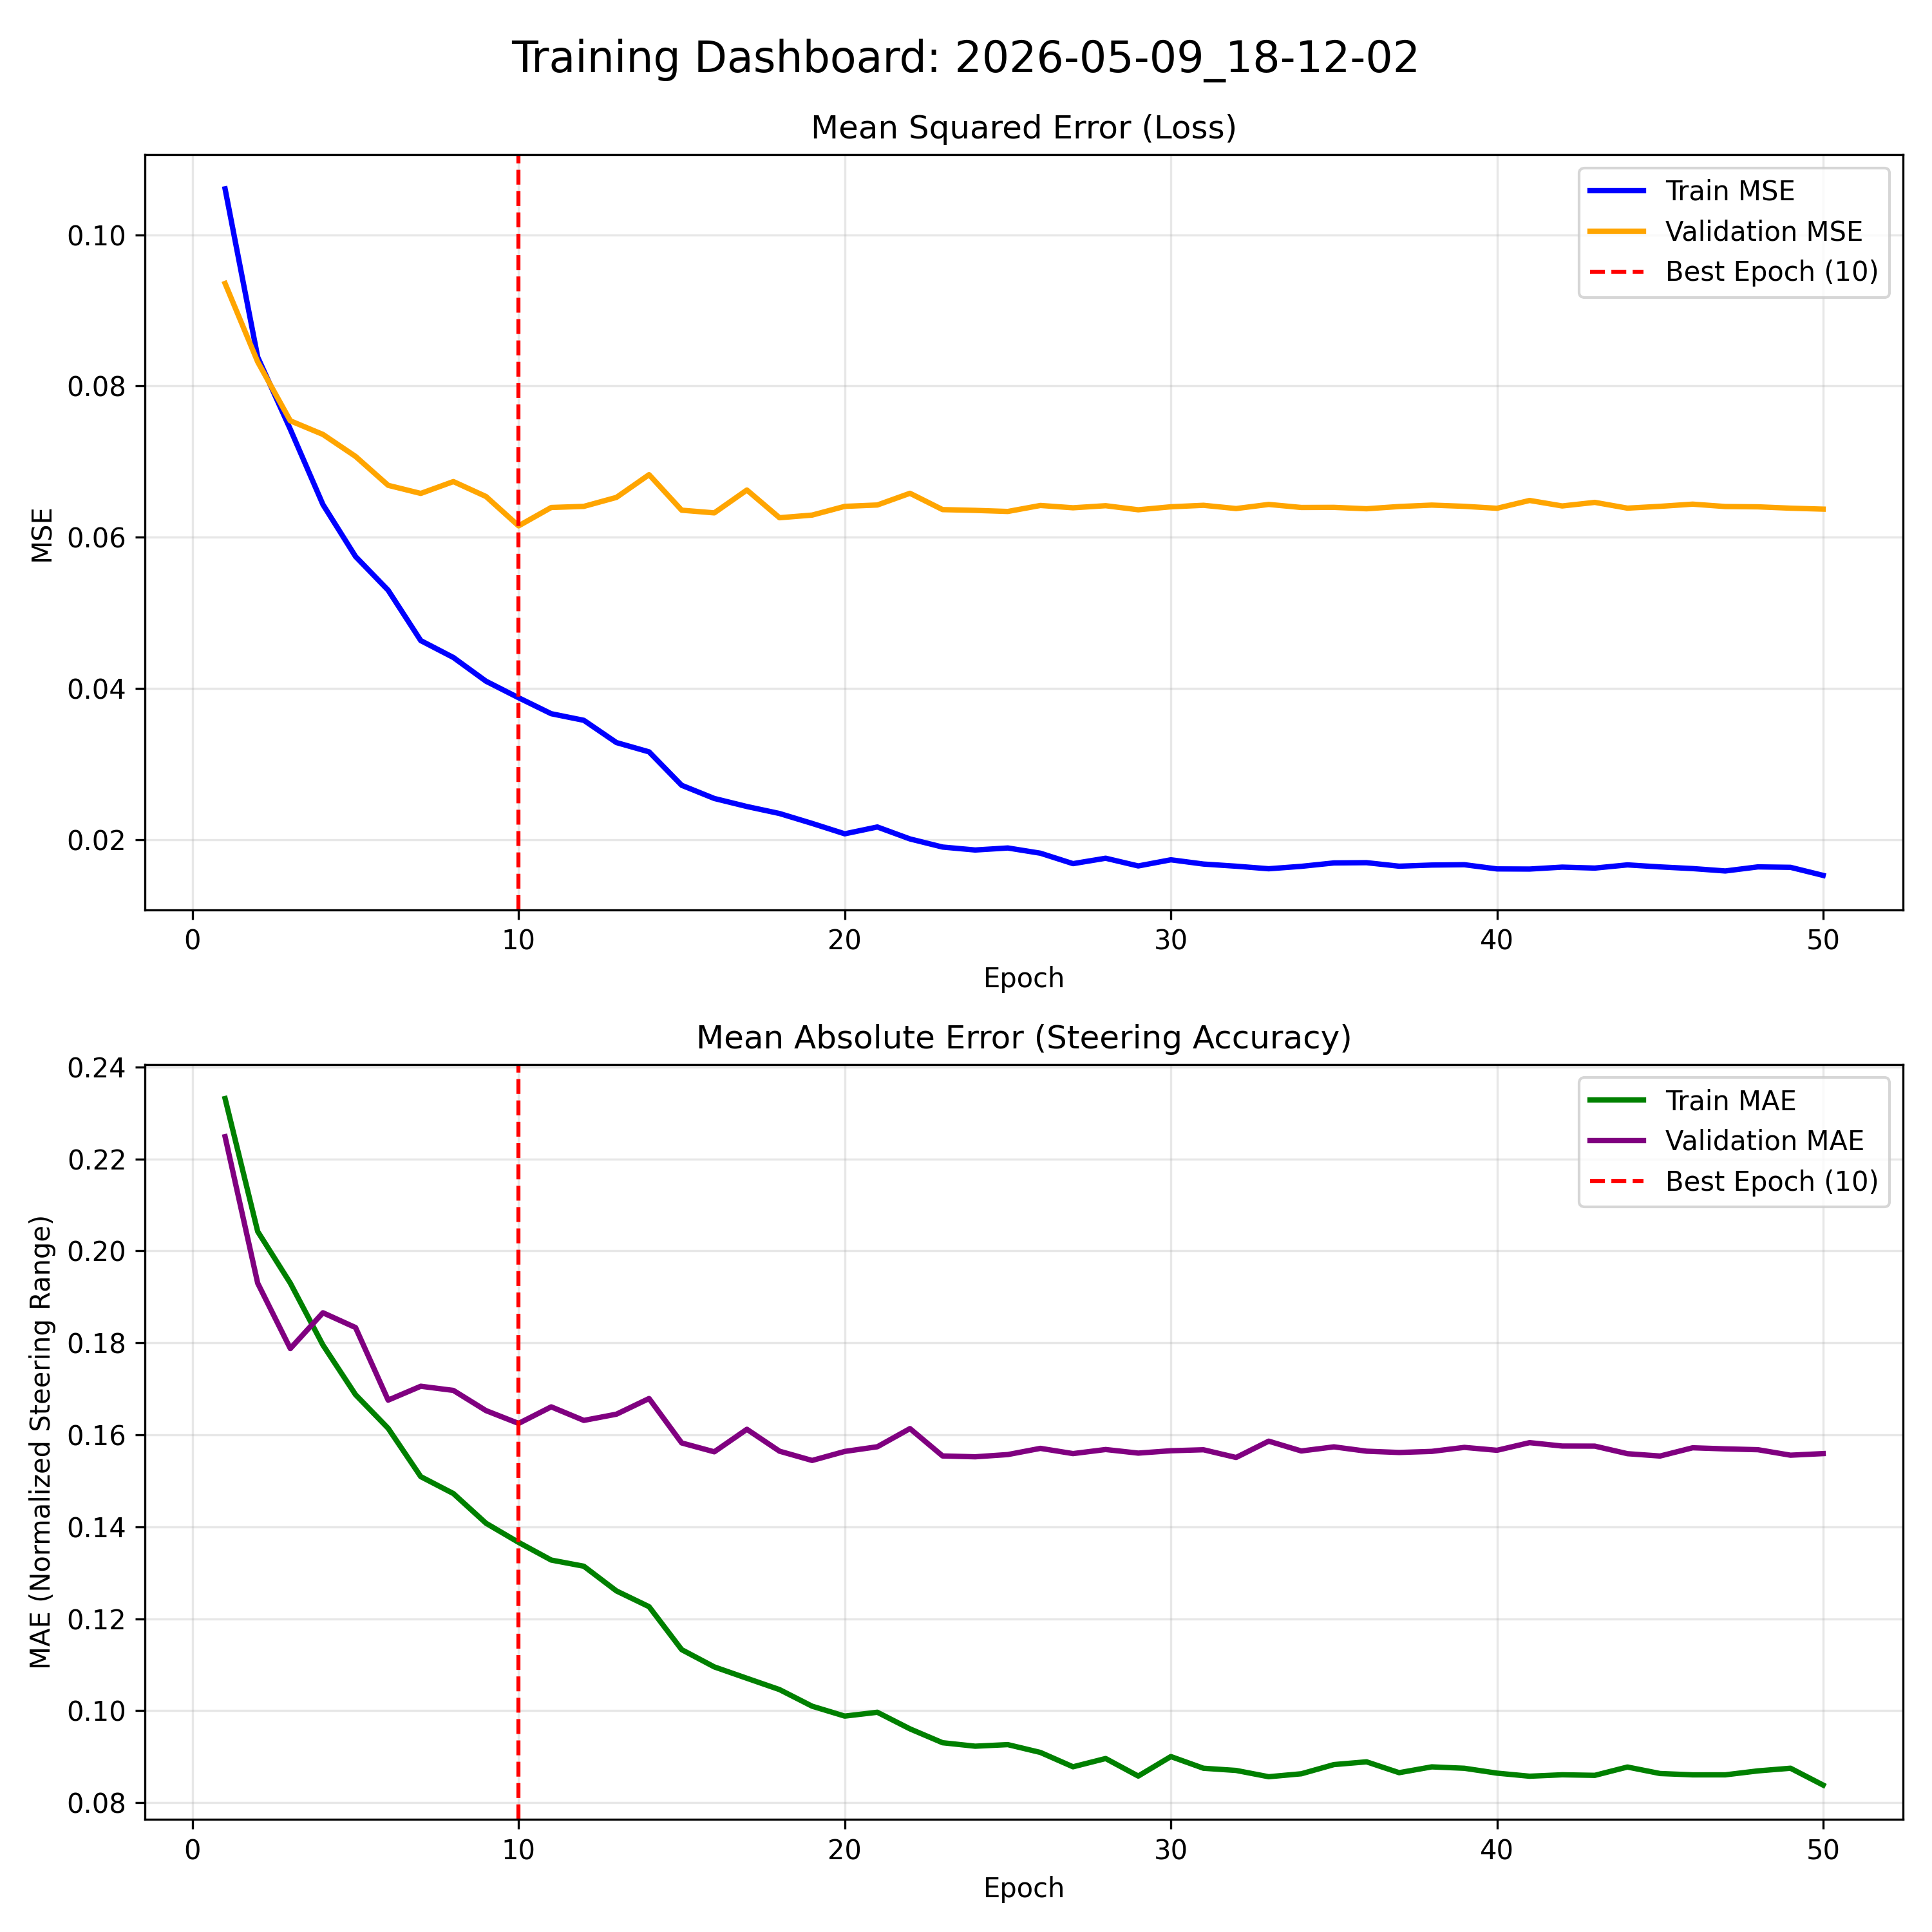
\includegraphics[width=1.0\linewidth]{chap4/images/best_model_metrics.png}
	\caption{The Egocentric Dynamic Crop Model's training profile showed stable convergence, with both MSE and MAE decreasing steadily without significant validation noise.}\label{fig:4.5}
\end{figure}

As shown in Figure~\ref{fig:4.5}, it quickly achieved a highly stable validation MSE of 0.0615 by Epoch 10. The entire optimization process was completed in just 2 minutes and 24 seconds, proving the model is both accurate and computationally lightweight.

\subsection{Real-World Navigation and Endurance}

The proposed Egocentric Model successfully guided the robot through the entire track.

\begin{figure}[H]
	\centering
	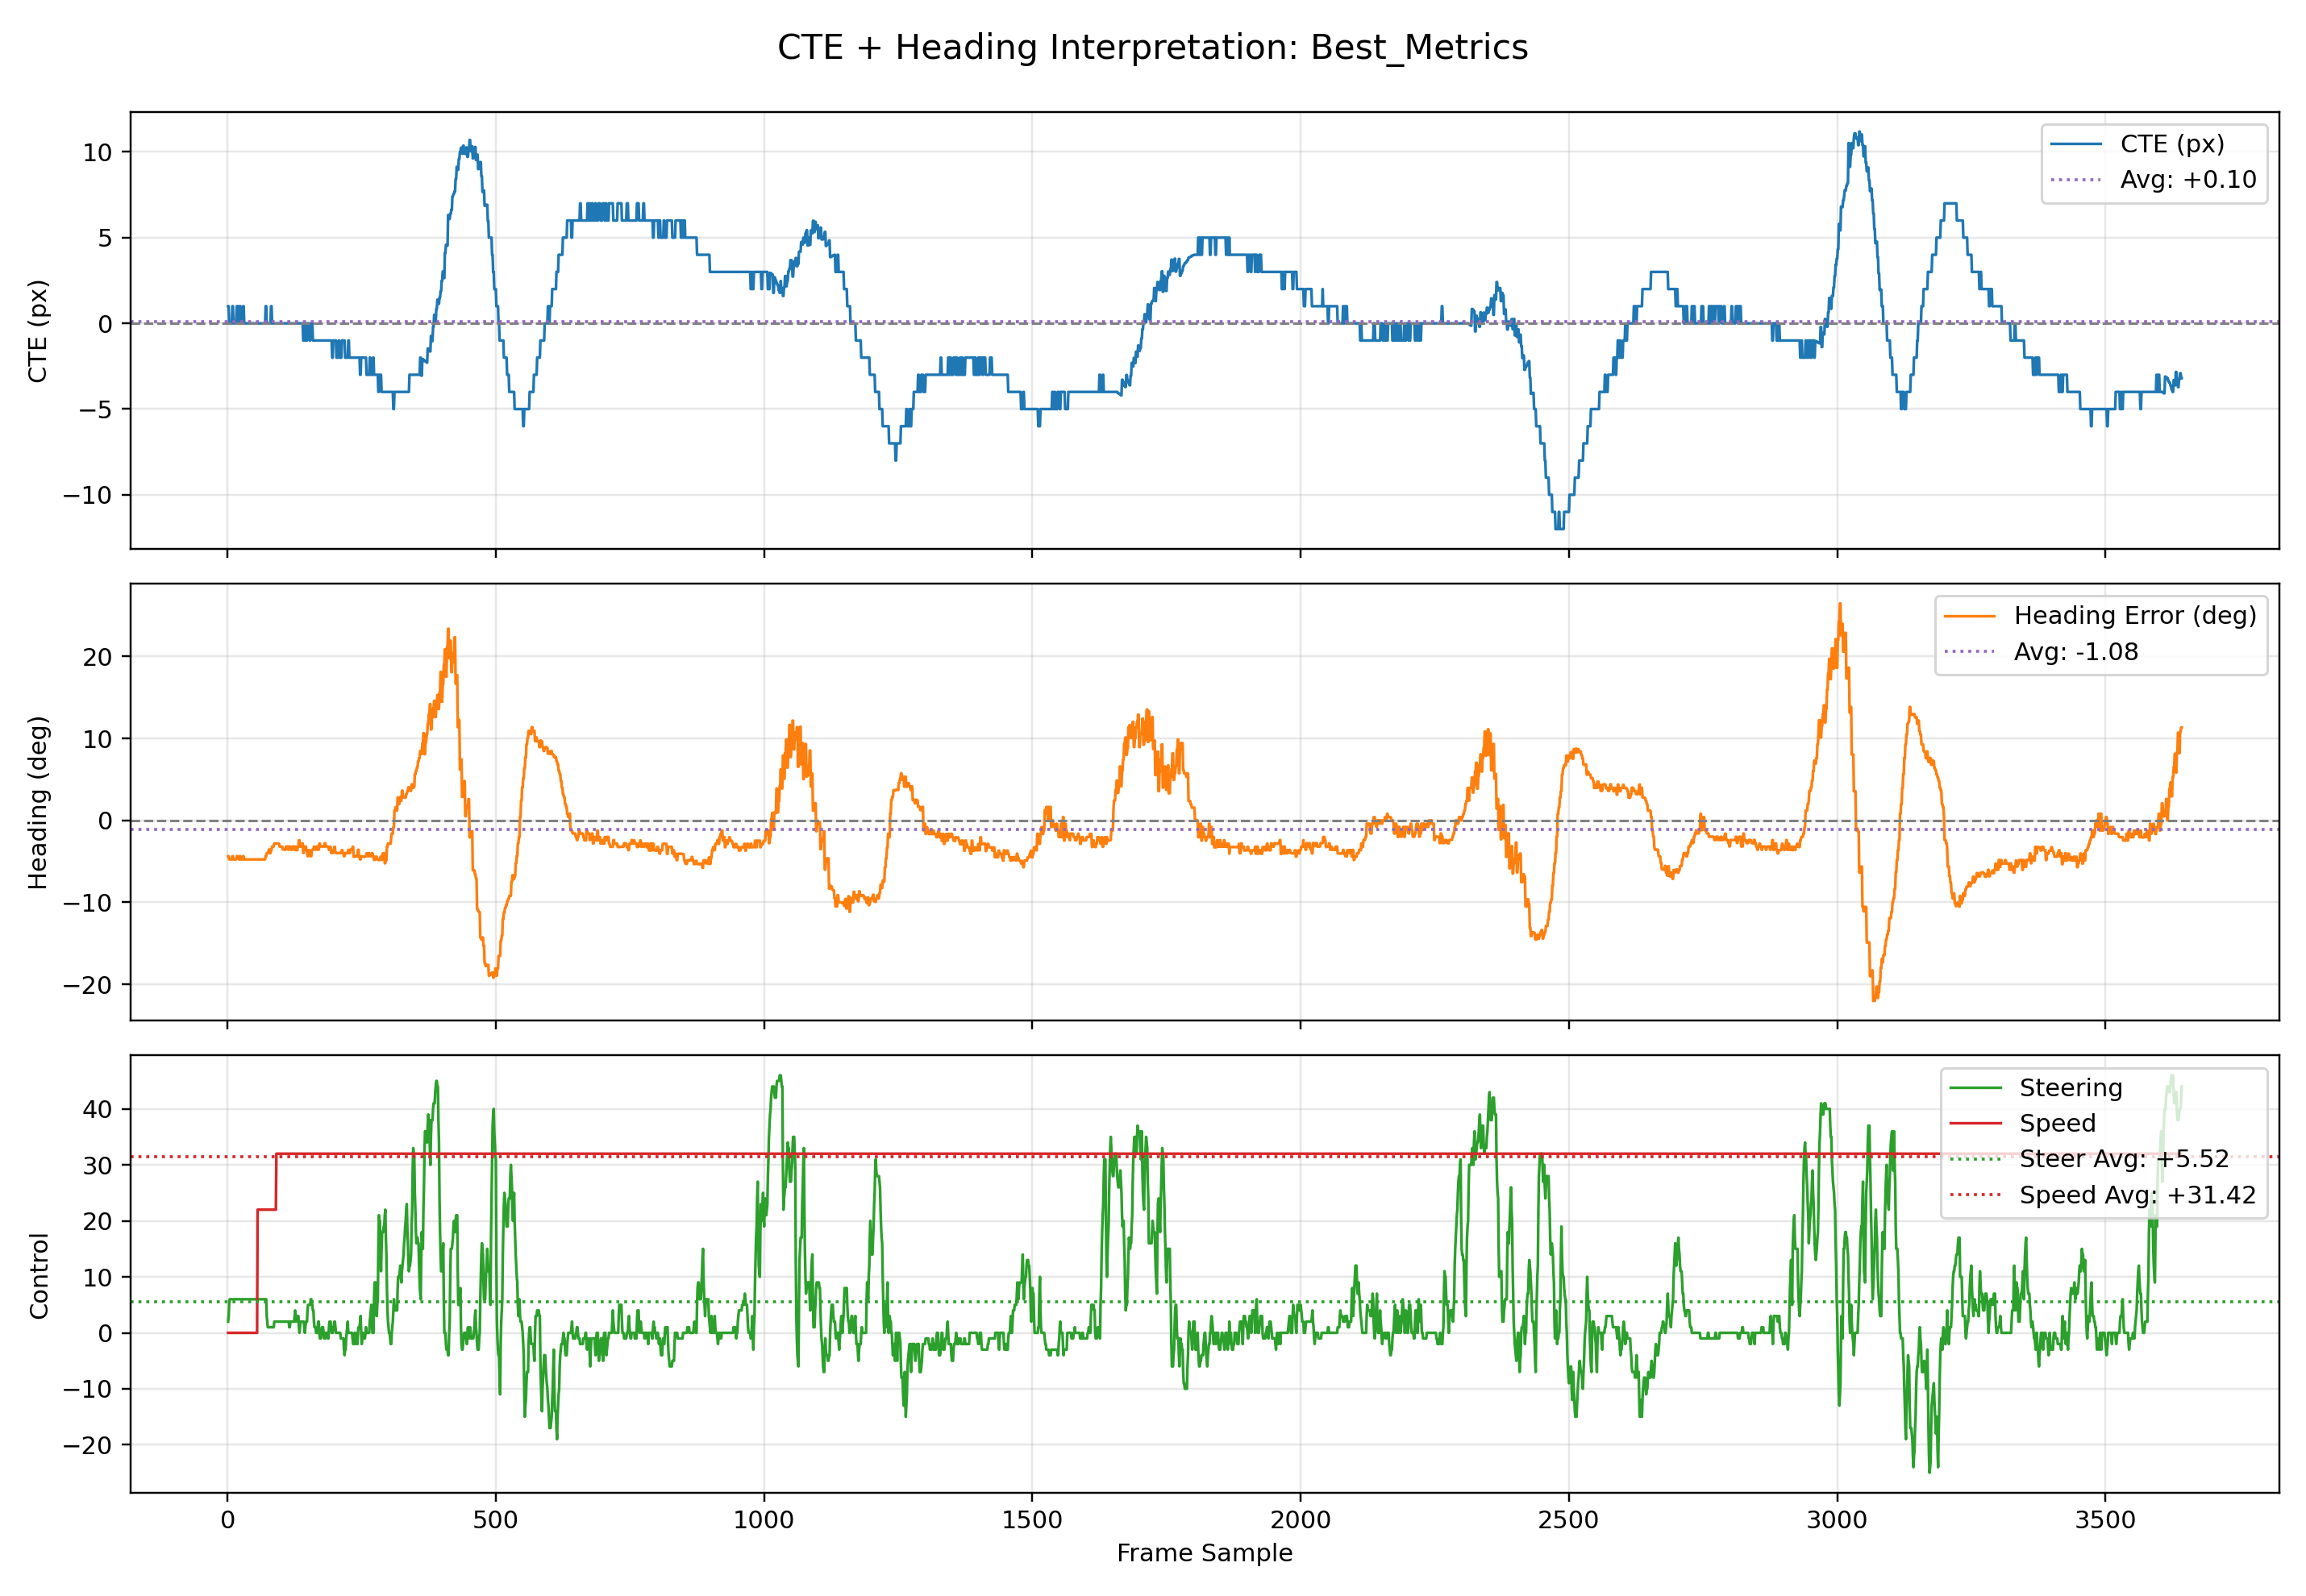
\includegraphics[width=1.0\linewidth]{chap4/images/Best_Metrics_interpretation.png}
	\caption{Physical deployment of the Egocentric Dynamic Crop Model resulted in successful navigation through the entire track, with stable CTE and Heading Error profiles.}\label{fig:4.6}
\end{figure}

Deployed over a continuous run of 3,642 frames, it achieved an extremely low tracking error with an RMSE of 4.0249 pixels and a Mean Absolute CTE of just 3.1700 pixels. The telemetry in Figure 4.6 demonstrates smooth, consistent steering across both straightaways and sharp turns without a single boundary breach.

\section{Comparative Tracking Performance}
Table~\ref{tab:4.1} and Figure~\ref{fig:4.7} summarize the final real-world tracking metrics across all three chronological iterations, clearly illustrating the dramatic stability improvements achieved by the egocentric crop.

\begin{table}[H]
\centering
\caption{Physical Track Testing Results Across All Iterations}
\label{tab:4.1}
\begin{tabularx}{\linewidth}{l X r X r}
\toprule
\textbf{Physical Trial} & \textbf{Active Model} & \textbf{Total Frames Survived} & \textbf{Track Outcome} & \textbf{CTE (RMSE, px)} \\
\midrule
Baseline A & Baseline A (Full AOI) & 636 & Drove off track & 30.9992 \\
Baseline B (Session 1) & Baseline B (Feature-Extracted) & 772 & Drove off track & 35.7224 \\
Baseline B (Session 2) & Baseline B (Feature-Extracted) & 1,122 & Drove off track & 84.3785 \\
Final System & Proposed Egocentric Model & 3,642 & Completed successfully & 4.0249 \\
\bottomrule
\end{tabularx}
\end{table}

\begin{figure}[H]
	\centering
	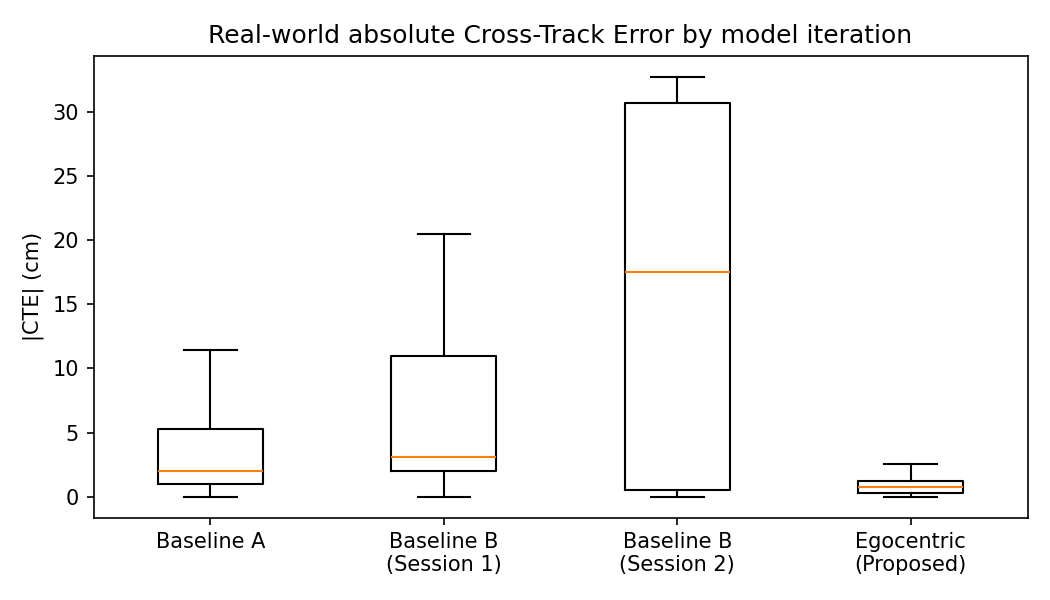
\includegraphics[width=1.0\linewidth]{chap4/images/absolute_cte_boxplot.png}
	\caption{Real-World Trajectory Deviations: Absolute Cross-Track Error Box Plot.}\label{fig:4.7}
\end{figure}
The box plot in Figure~\ref{fig:4.7} shows a dramatic contraction of the error distribution for the proposed model, with a much lower median and tighter interquartile range than Baselines A and B. This indicates not only lower average tracking error but also substantially reduced variability and fewer large deviations.

\section{In-Depth Performance of the Model}
To comprehensively validate the proposed end-to-end architecture, the Egocentric Dynamic Crop model was evaluated across three specific track topologies of increasing B{\'e}zier curve complexity. By entirely removing the PID control components and relying strictly on the Convolutional Neural Network (CNN) for high-level navigation, this phase of testing isolates the controller's ability to dynamically scale continuous steering outputs based solely on visual geometric features.

\subsection{Statistical Analysis Methodology}
For each evaluation scenario, the robot was deployed in a continuous autonomous run during which the tracking system recorded per-frame Cross-Track Error (CTE) and Heading Error at approximately 60~Hz. To evaluate tracking consistency over sustained periods, telemetry is resolved per \emph{lap} rather than over arbitrary fixed-length frame windows. A lap represents one complete physical circuit of the track, aligning each consistency window with a meaningful unit of the course rather than a time-slice that spans variable parts of a circuit. Laps are partitioned by dividing the total duration of each scenario by the number of complete laps. Mirroring the policy of excluding incomplete segments, partial trailing laps (e.g., the final 14.3~s of the Scenario 3 run) are discarded so that only complete circuits contribute. The full quantitative summary is presented in Tables~\ref{tab:4.2}, \ref{tab:per_lap_consistency}, and \ref{tab:per_lap_detail}.

All cross-track errors are measured in the rectified bird's-eye-view canvas, which spans $800 \times 800$~pixels and maps to the physical arena of approximately $2.0$--$3.0$~m per side. Adopting a nominal arena width of $2.5$~m yields a scale of approximately $0.31$~cm per pixel, which is used throughout this chapter to report approximate real-world deviations alongside the pixel measurements. Because the physical arena dimension is approximate, the centimetre figures are likewise approximate (to within roughly $\pm 20\%$). The steering command reported throughout is the raw controller command after scaling the network's normalized output (scaling gain $k_{steer}=50$, clipped to $[-50,50]$), where positive values denote rightward turns and negative values leftward turns. Commands between $-2$ and $2$ are treated as straight-line driving (deadband). Empirically, this raw command maps monotonically to the robot's measured yaw rate and saturates at high-magnitude commands as the differential-drive platform reaches its motor limits; the values are therefore reported as unitless command magnitudes rather than physical angles.

\begin{table}[H]
\centering
\caption{Kinematic Performance Summary of the Final Egocentric Model}
\label{tab:4.2}
\footnotesize
\begin{tabularx}{\linewidth}{@{}l X r r r r@{}}
\toprule
 & & & \multicolumn{3}{c@{}}{\textbf{Cross-Track Error (px)}} \\
\cmidrule(l){4-6}
\textbf{Scenario} & \textbf{Track Topology} & \textbf{Frames} & \textbf{Mean $\pm$ SD} & \textbf{RMSE} & \textbf{P95} \\
\midrule
1 & 45$^\circ$ B{\'e}zier curves & 2{,}934 & 1.91 $\pm$ 1.84 & 2.66 & 5.0 \\
2 & 90$^\circ$ square path & 1{,}709 & 2.74 $\pm$ 2.23 & 3.54 & 8.0 \\
3 & 180$^\circ$ sustained U-turn & 13{,}421 & 5.07 $\pm$ 4.62 & 6.86 & 15.0 \\
\bottomrule
\end{tabularx}
\end{table}

% chap4/per_lap_consistency.tex
% Trial-to-trial CTE RMSE consistency over N=10 independent randomized-start trials per scenario.
% Replaces the old per-lap (within-one-run) analysis. \input this into Chapter 4.

\subsection{Trial-to-Trial Tracking Consistency}
\label{sec:per_lap_consistency}
Because each evaluation trial is exactly one circuit of the track, the repeated unit is the
\emph{independent trial} rather than a lap within a continuous run. Tracking consistency is therefore
reported as the distribution of per-trial CTE RMSE across the $N=10$ randomized-start trials of each
scenario (Table~\ref{tab:per_lap_consistency}).

\begin{table}[H]
\centering
\caption{Trial-to-trial CTE RMSE consistency ($N=10$ independent randomized-start trials per scenario).}
\label{tab:per_lap_consistency}
\footnotesize
\begin{tabular}{@{}l r r r@{}}
\toprule
\textbf{Scenario} & \textbf{Trials ($n$)} & \textbf{Per-trial RMSE mean $\pm$ SD (cm)} & \textbf{Range (cm)} \\
\midrule
1 (45$^\circ$)   & 10 & 0.98 $\pm$ 0.11 & 0.76--1.15 \\
2 (90$^\circ$)   & 10 & 1.49 $\pm$ 0.14 & 1.26--1.69 \\
3 (180$^\circ$)  & 10 & 0.91 $\pm$ 0.04 & 0.86--0.96 \\
4 (held-out)     & 10 & 2.04 $\pm$ 0.16 & 1.77--2.44 \\
\bottomrule
\end{tabular}
\end{table}

The small standard deviations (0.04--0.17~cm) are the central result: the controller produces
near-identical tracking error across independent trials that each start from a different randomized
pose, indicating high repeatability rather than a single lucky run. The trained-track scenarios
(1--3) cluster tightly, while the held-out track (Scenario~4) shows both a higher mean and a wider
spread, consistent with the generalization gap reported in Section~\ref{sec:generalization}.


\subsection{Scenario 1: 45-Degree B{\'e}zier Curves}
The first scenario tests mild, continuous curvature over 2{,}934 frames (49.0~s) of continuous autonomous driving. Rather than exhibiting the fishtailing or oscillatory steering behavior commonly observed in pure behavioral cloning models without derivative damping, the model demonstrated highly anticipatory steering. As the $45^\circ$ curves entered the egocentric bounding box, the convolutional feature extractor registered the gradual geometric shift, resulting in a smooth, continuous adjustment of the steering vector. The model achieved a mean absolute CTE of \textbf{1.91 $\pm$ 1.84}~px (RMSE = 2.66~px, $\approx 0.83$~cm), with 95\% of all frames remaining within 5.0~px ($\approx 1.6$~cm) of the reference path. Per-lap consistency analysis across 10 completed laps yielded a mean per-lap RMSE of \textbf{2.28 $\pm$ 1.37}~px (range: 0.93--4.73~px, Table~\ref{tab:per_lap_consistency}), confirming consistent tracking throughout the run. The Heading Error remained bounded, with a mean of $-1.05 \pm 5.13^\circ$ and peaking at \textbf{31.92$^\circ$} at the sharpest point of the transition, proving that the model does not overreact to gentle path deviations and smoothly tracks shallow curves.

\subsection{Scenario 2: 90-Degree B{\'e}zier Corners (Square Path)}
Navigating the square path over 1{,}709 frames (28.5~s) tested the model's response to rapid, orthogonal geometric changes. The model achieved a mean absolute CTE of \textbf{2.74 $\pm$ 2.23}~px (RMSE = 3.54~px, $\approx 1.1$~cm), with 95\% of frames within 8.0~px ($\approx 2.5$~cm) of the reference path. The Heading Error remained bounded, with a mean of $-3.16 \pm 5.74^\circ$ and a peak magnitude of $20.98^\circ$. Approaching a $90^\circ$ corner requires a sharp spike in actuation. Upon entering the apex of the corners, the model successfully executed aggressive, high-magnitude steering commands, reaching a peak raw steering command magnitude of \textbf{33.0}.

\begin{figure}[H]
	\centering
	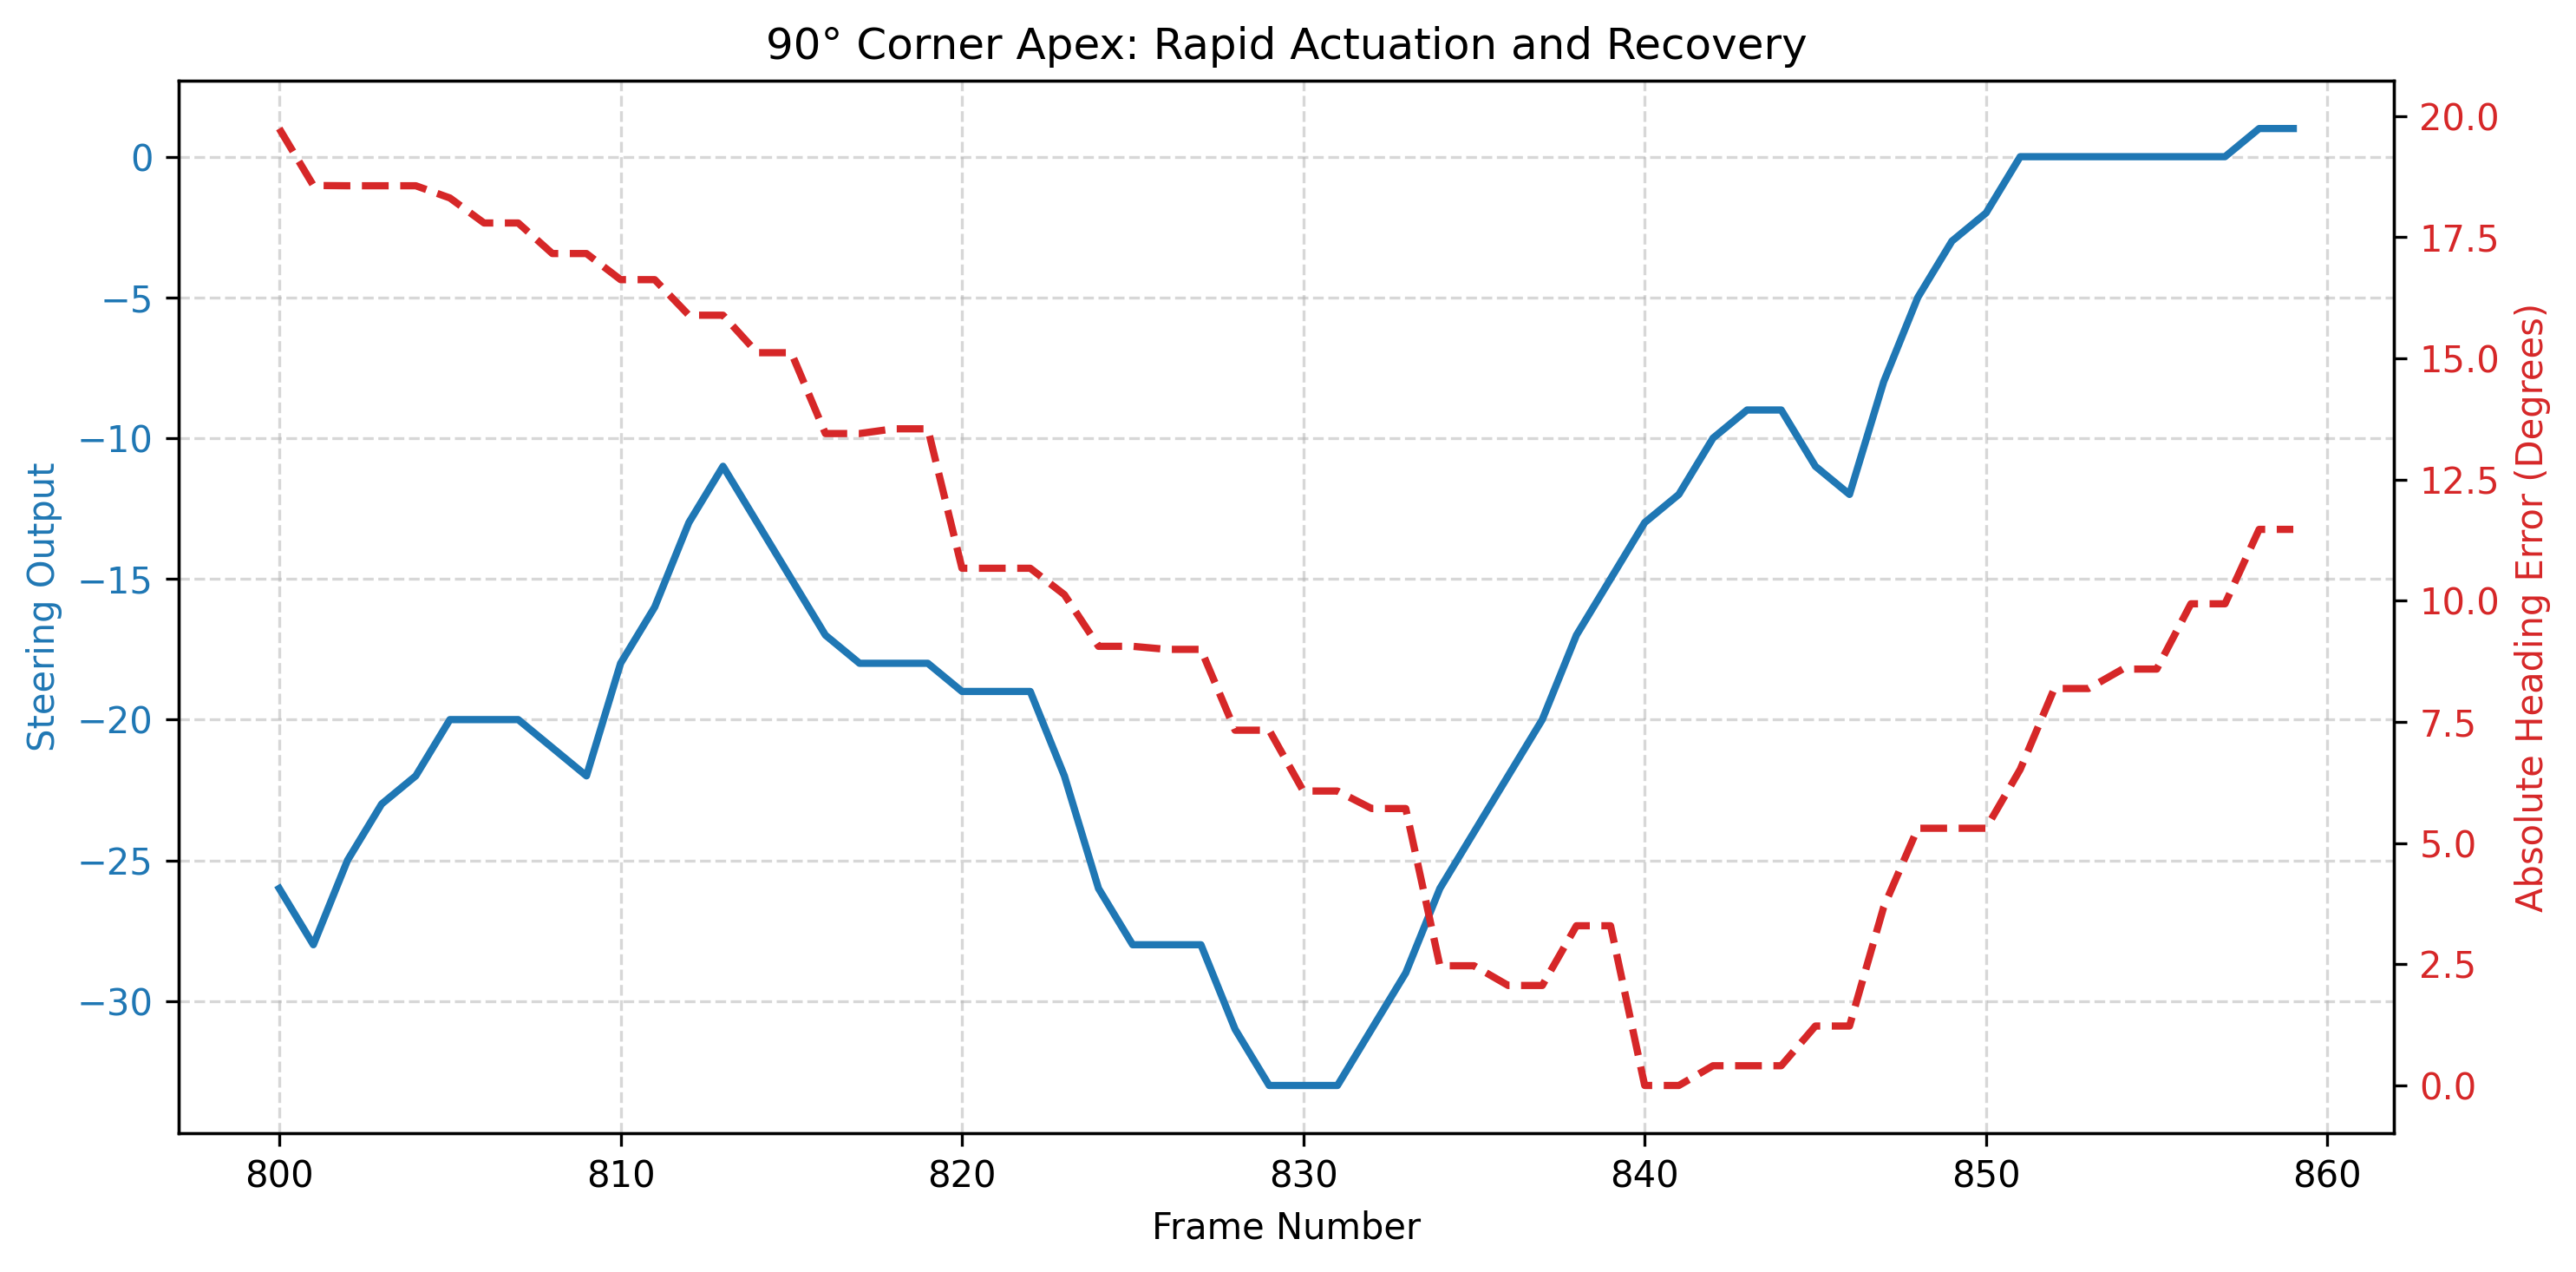
\includegraphics[width=1.0\linewidth]{chap4/images/90_Degree_Telemetry.png}
	\caption{90-degree cornering telemetry showing rapid actuation and recovery under orthogonal curvature.}\label{fig:4.8}
\end{figure}

Importantly, as visualized in Figure~\ref{fig:4.8}, the Egocentric Dynamic Crop ensured that the path boundaries remained centered in the network's view rather than sweeping out of frame. This continuous recentering allowed for a rapid and stable recovery; the model brought the heading error back down to $0^\circ$ within just \textbf{11 frames} (approximately \textbf{0.73 s} at a 15 Hz operating frequency) upon exiting the corner, resuming straight-line stability instantly.

\subsection{Scenario 3: 180-Degree Sustained U-Turns}
The final topology tested the system's kinematic endurance during extreme, continuous curvature. This scenario produced the longest continuous run at 13{,}421 frames over 226.5~s (approximately 3.8 minutes) of uninterrupted autonomous driving, encompassing many complete laps of the U-turn track. During the 180-degree U-turns, the model was forced to hold a near-maximum steering angle for a prolonged period.

\begin{figure}[H]
	\centering
	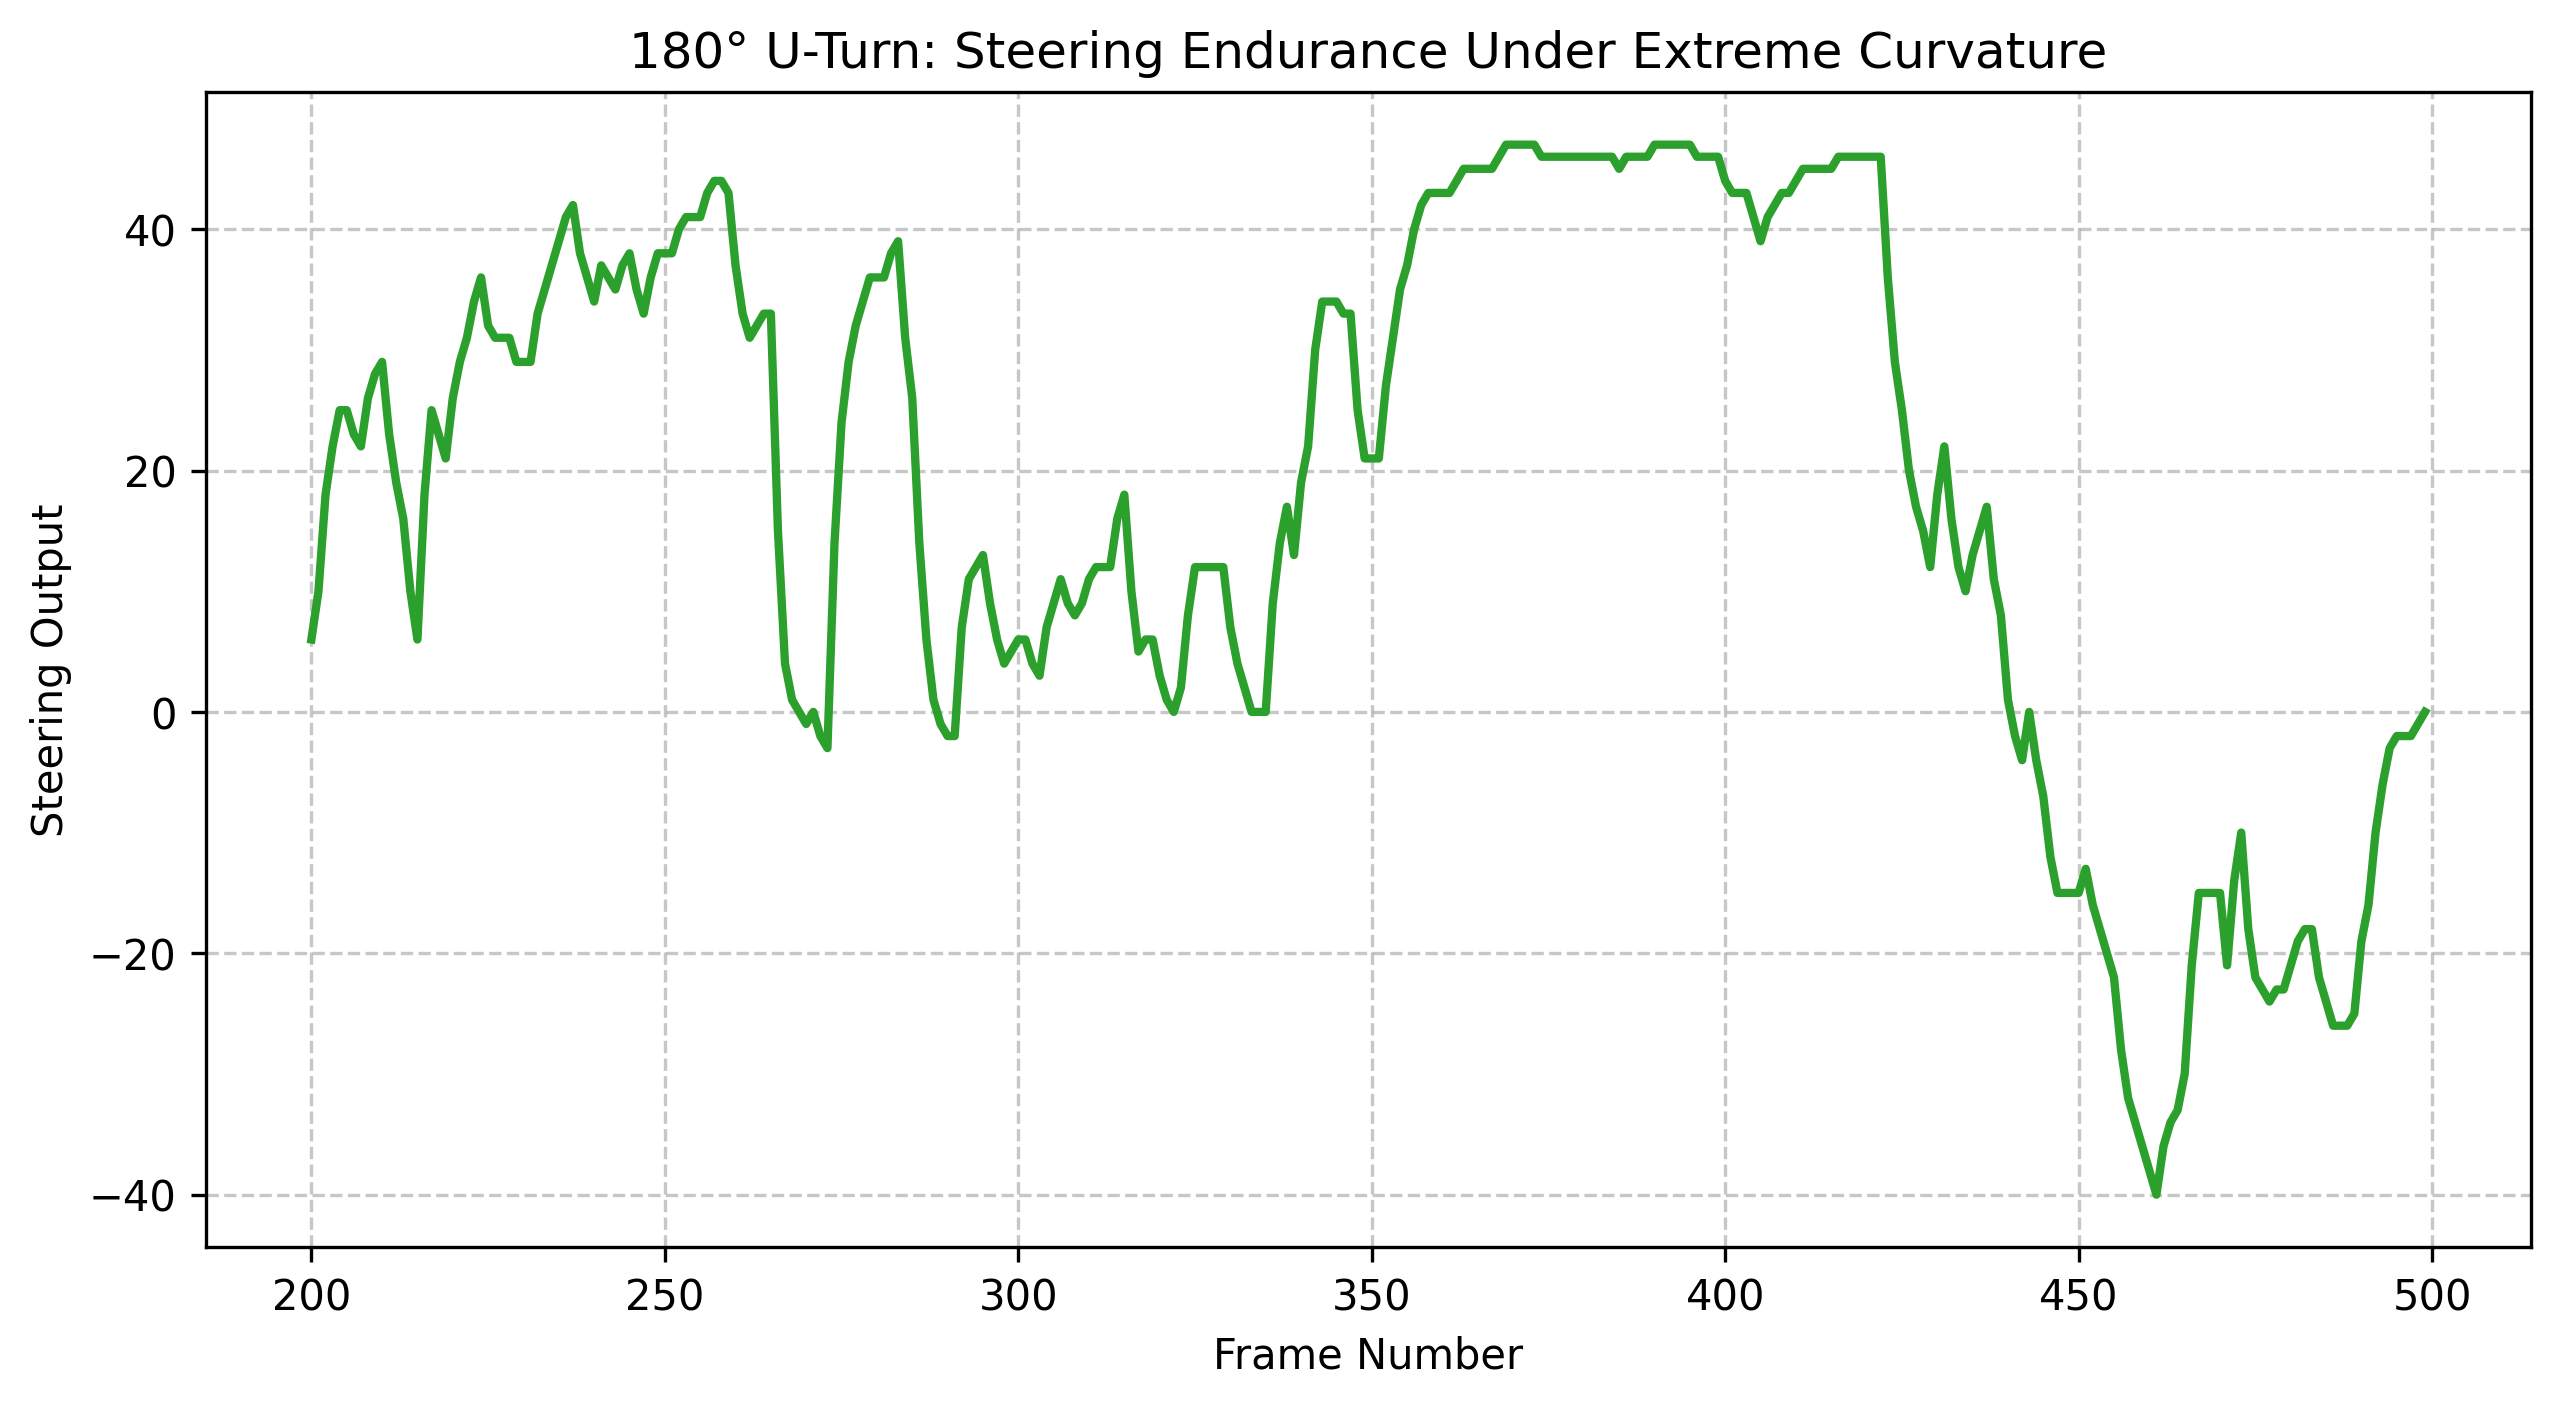
\includegraphics[width=1.0\linewidth]{chap4/images/180_Degree_Endurance.png}
	\caption{180-degree U-turn telemetry illustrating sustained steering actuation under extreme curvature.}\label{fig:4.9}
\end{figure}

The telemetry in Figure~\ref{fig:4.9} confirms that the network successfully handled the extreme geometric distortion, scaling up its actuation to reach and sustain a maximum raw steering command magnitude of \textbf{47.0}. The model achieved a mean absolute CTE of \textbf{5.07 $\pm$ 4.62}~px (RMSE = 6.86~px, $\approx 2.1$~cm), with 95\% of frames within 15.0~px ($\approx 4.7$~cm) of the reference path and a worst-case deviation of 28.9~px ($\approx 9.0$~cm), which remains below half the chassis width. The Heading Error over the run had a mean of $-0.16 \pm 9.34^\circ$ with a peak magnitude of $33.95^\circ$. Per-lap consistency analysis across 8 completed laps yielded a mean per-lap RMSE of \textbf{6.56 $\pm$ 2.08}~px (range: 4.43--10.14~px, Table~\ref{tab:per_lap_consistency}), demonstrating that tracking performance remained bounded throughout the extended run despite the extreme curvature. This confirms that the CNN effectively learned the structural rules of extreme curvature tracking without requiring a rigid mathematical path-planning algorithm.

\begin{figure}[H]
	\centering
	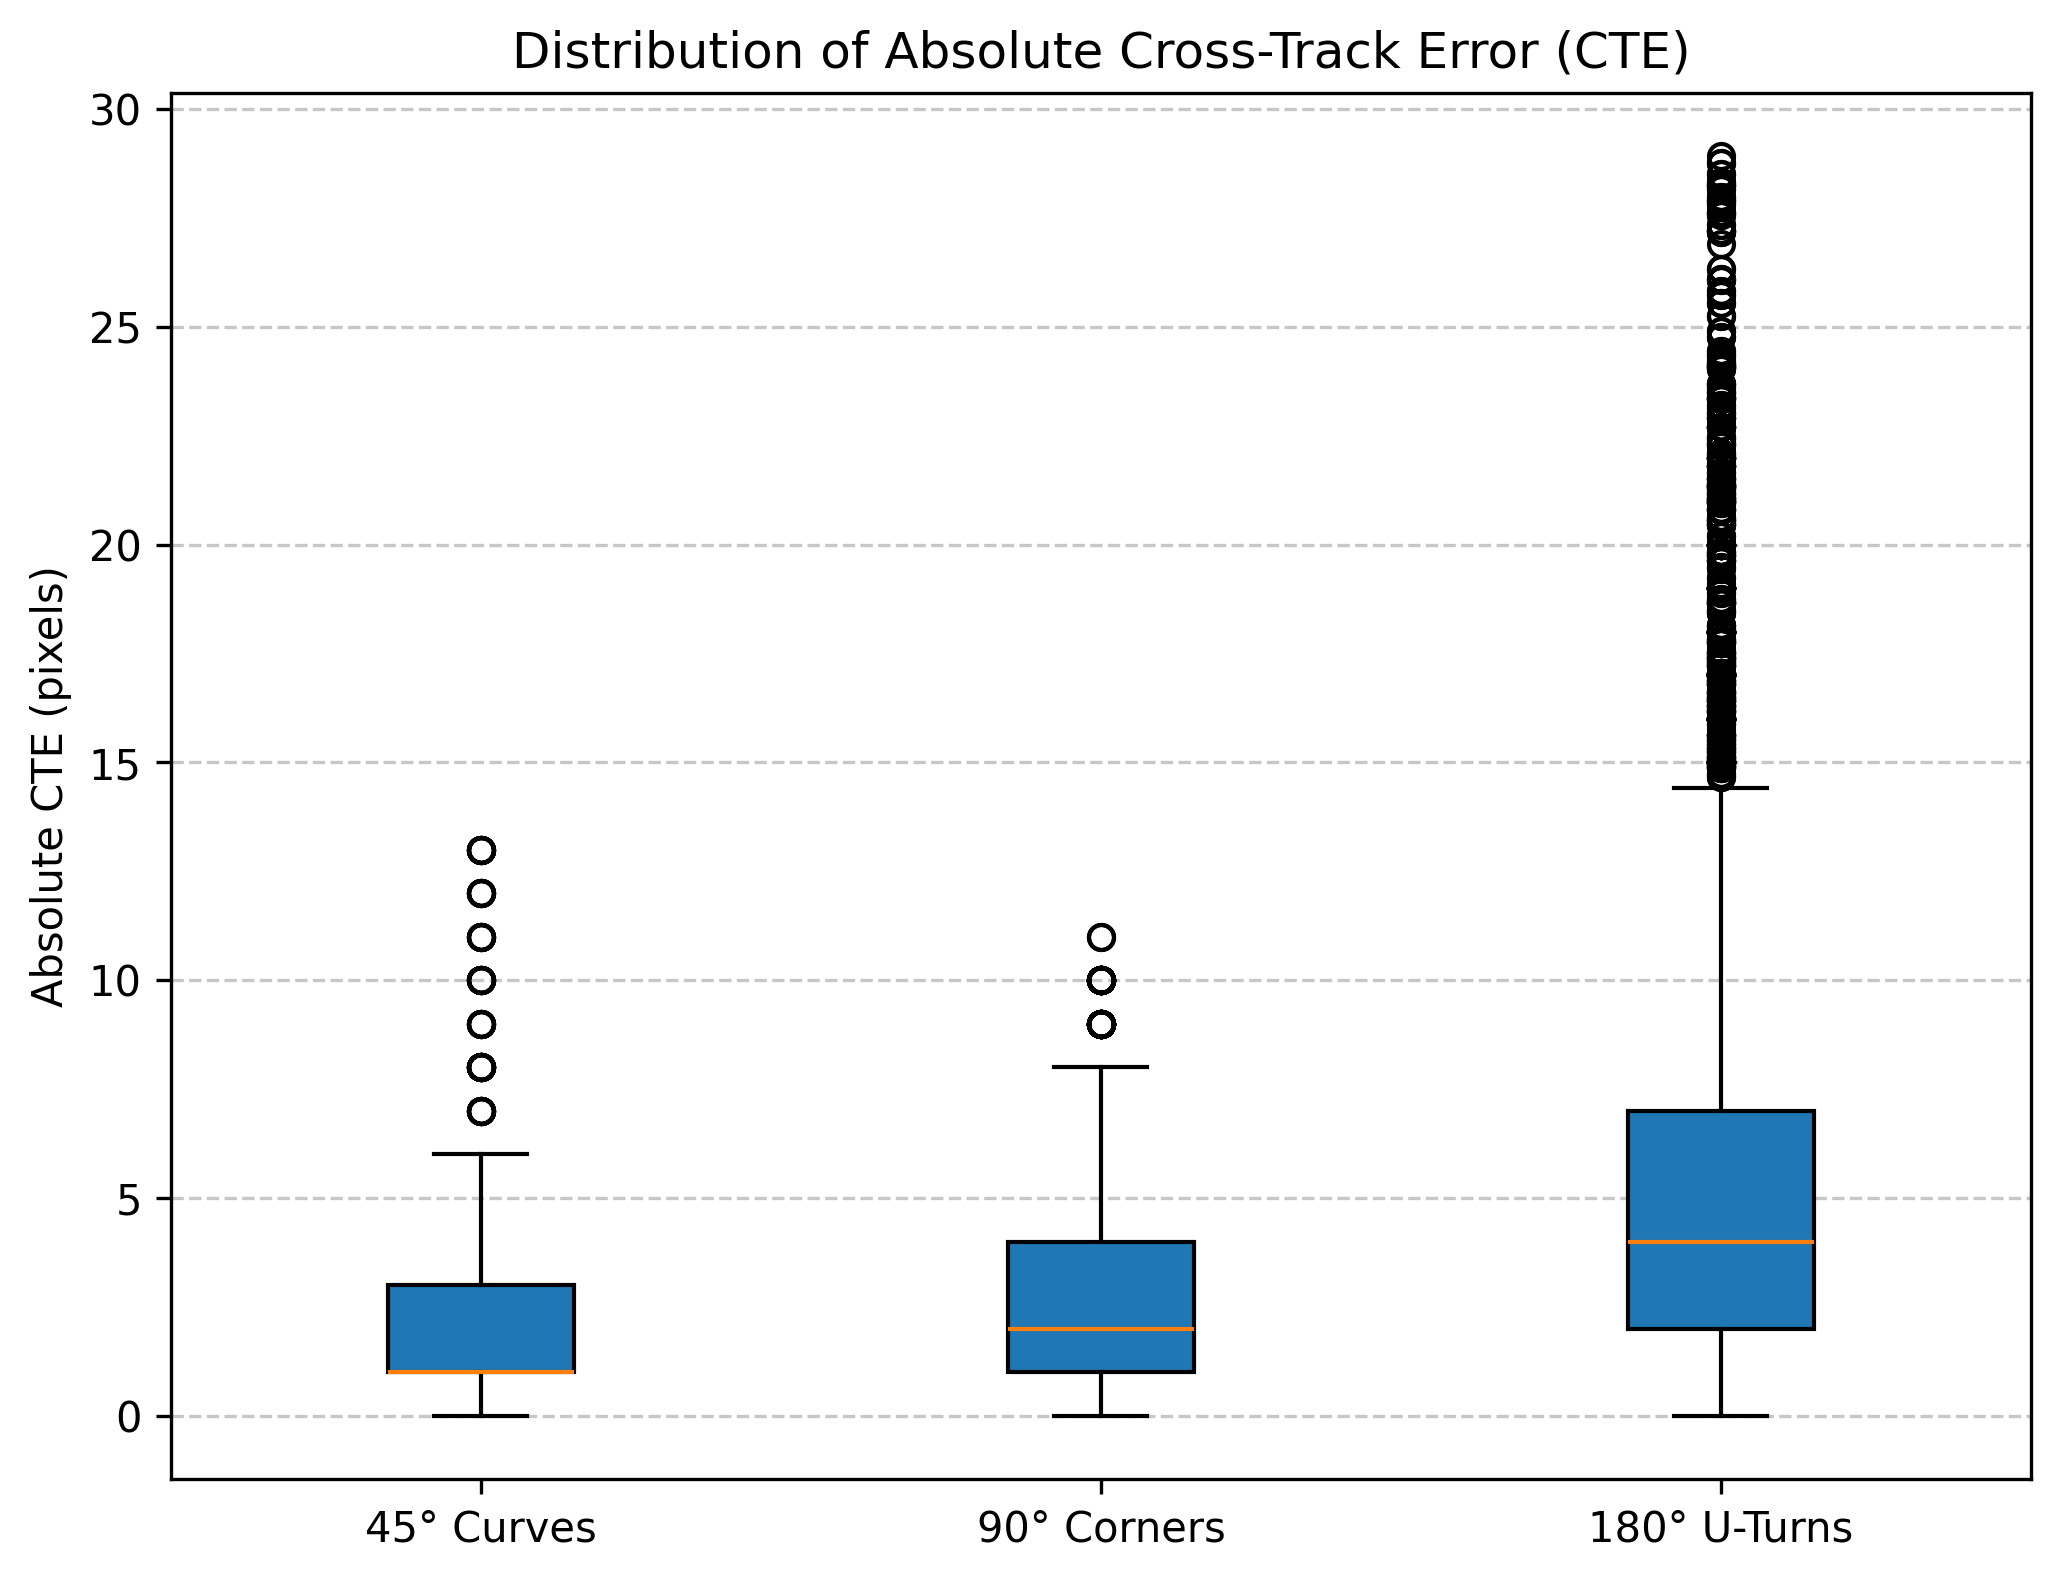
\includegraphics[width=1.0\linewidth]{chap4/images/CTE_Boxplot.png}
	\caption{Distribution of Absolute Cross-Track Error (CTE) across varying B{\'e}zier curve complexities, demonstrating bounded error scaling under extreme geometric distortion.}\label{fig:4.10}
\end{figure}

\section{Control Decision Discretization and Confusion Matrix}
To evaluate the directional correctness of steering decisions issued by the end-to-end CNN, the continuous telemetry logs were mapped to discrete control states. Under the system's sign convention, positive values denote rightward sense for both quantities: a positive CTE indicates the robot is displaced to the \emph{right} of the reference path, and a positive steering command drives a rightward turn. Consequently, a positive CTE calls for a corrective \emph{leftward} steering action. The desired corrective action is therefore defined from the lateral displacement (CTE) as:

\begin{equation}
\text{Desired Action} =
\begin{cases}
\text{Left}, & \text{if } \text{CTE} > 2.0\text{ px} \\
\text{Straight}, & \text{if } -2.0\text{ px} \le \text{CTE} \le 2.0\text{ px} \\
\text{Right}, & \text{if } \text{CTE} < -2.0\text{ px}
\end{cases}
\end{equation}

The executed CNN control action is discretized from the raw steering command using the same $\pm 2.0$ dead-band, with commands greater than $+2.0$ classified as Right, those below $-2.0$ as Left, and those in between as Straight. With this convention, the matrix diagonal corresponds to correct corrective steering. The combined confusion matrix across all three track topologies is shown in Figure~\ref{fig:4.11}.

\begin{figure}[H]
	\centering
	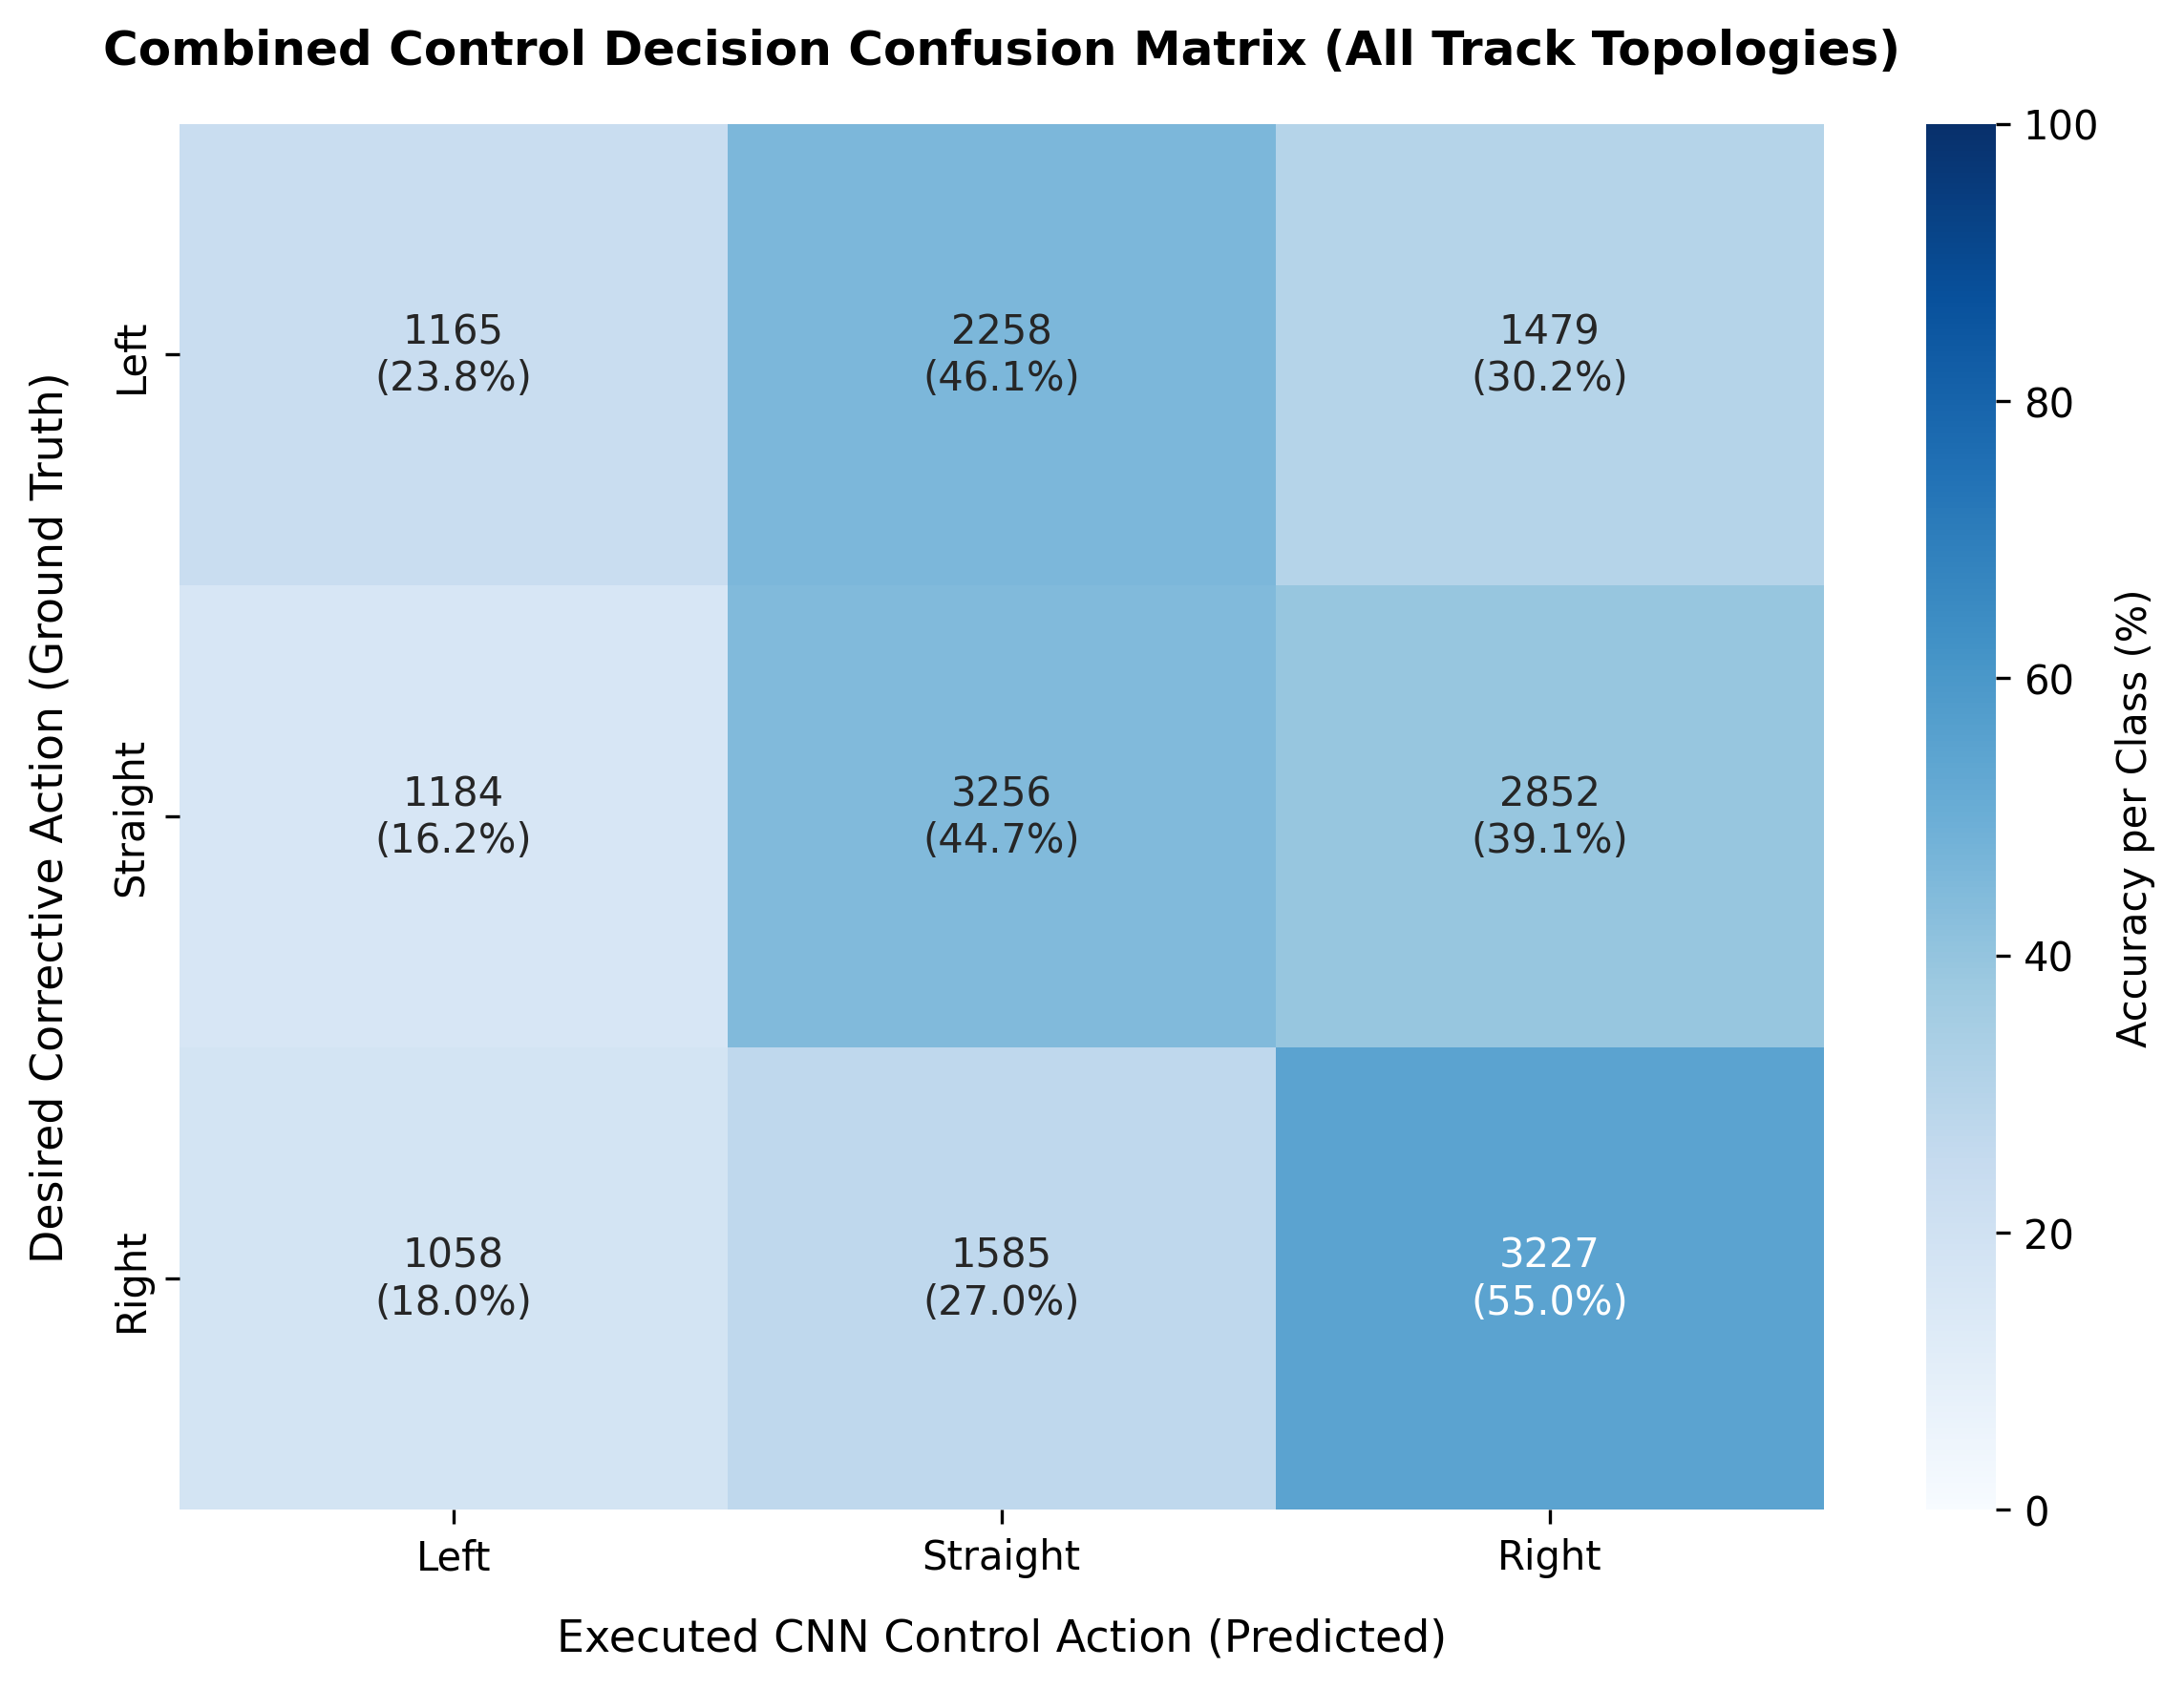
\includegraphics[width=0.82\linewidth]{chap4/images/confusion_matrix_combined.png}
	\caption{Combined Control Decision Confusion Matrix across all track topologies. The matrix maps cross-track error states to the corresponding steering actions.}\label{fig:4.11}
\end{figure}

A key control-theoretic observation is the \textit{Proactive Curve-Following Paradox}. When tracking a curve accurately, the controller holds the vehicle near the centerline (ground truth classified as Straight) while still executing active left or right steering to follow the upcoming geometry. The resulting label mismatch does not indicate failure; it demonstrates anticipatory, feedforward trajectory planning rather than a purely reactive corrective policy.